% English-only project. Chinese \zhpara passages removed from main.tex.
%% 
%% Copyright 2019-2024 Elsevier Ltd
%% 
%% Version 2.4
%% 
%% This file is part of the 'CAS Bundle'.
%% --------------------------------------
%% 
%% It may be distributed under the conditions of the LaTeX Project Public
%% License, either version 1.2 of this license or (at your option) any
%% later version.  The latest version of this license is in
%%    http://www.latex-project.org/lppl.txt
%% and version 1.2 or later is part of all distributions of LaTeX
%% version 1999/12/01 or later.
%% 
%% The list of all files belonging to the 'CAS Bundle' is
%% given in the file `manifest.txt'.
%% 
%% Template article for cas-dc documentclass for 
%% double column output.

\PassOptionsToPackage{no-math}{fontspec}
\documentclass[a4paper,fleqn]{cas-dc}
% cas-common calls \vbox_unpack_clear:N, removed from current expl3.
\ExplSyntaxOn
\cs_if_exist:NF \vbox_unpack_clear:N
  { \cs_new_protected:Npn \vbox_unpack_clear:N #1 { \vbox_unpack_drop:N #1 } }
\ExplSyntaxOff

% Allow continuous Type1 scaling (STIX/.fd discrete sizes → ≤0.5pt substitution warning)
\usepackage{anyfontsize}

%\usepackage[authoryear,longnamesfirst]{natbib}
%\usepackage[authoryear]{natbib}
\usepackage[numbers]{natbib}
\usepackage{array}

%%%Author definitions
\def\tsc#1{\csdef{#1}{\textsc{\lowercase{#1}}\xspace}}
\tsc{WGM}
\tsc{QE}
\tsc{EP}
\tsc{PMS}
\tsc{BEC}
\tsc{DE}
%%%Mine

\DeclareMathOperator*{\argmax}{arg\,max}
\DeclareMathOperator*{\argmin}{arg\,min}
\usepackage[ruled,vlined]{algorithm2e}
\DontPrintSemicolon
\SetAlFnt{\footnotesize}
\SetAlCapFnt{\footnotesize}
\SetAlCapNameFnt{\footnotesize\bfseries}
\SetAlgoSkip{bigskip}
\SetInd{0.4em}{0.7em}
\SetCommentSty{textit}
\hypersetup{
  colorlinks=False,
  citecolor=Violet,
  linkcolor=Red,
  urlcolor=Blue}

\usepackage{tabularx}
\usepackage{multirow}
\usepackage{makecell}
\usepackage{booktabs}
\usepackage{subcaption}
\captionsetup{font={small,rm},labelfont={bf,rm}}
\usepackage{xcolor}
\usepackage{soul}
\usepackage{amsthm}
\usepackage{amsmath}
\usepackage{fontspec}
% All text fonts (roman, sans, and mono) in Times New Roman, so that body text,
% headings, captions, headers/footers, tables, and \texttt{} identifiers match.
% Falls back to the bundled Latin Modern fonts where Times New Roman is absent.
% (Mathematical symbols keep the class math font.)
\IfFontExistsTF{Times New Roman}
  {\setmainfont{Times New Roman}
   \setsansfont{Times New Roman}
   \setmonofont{Times New Roman}}
  {\setmainfont{lmroman10-regular.otf}
   \setsansfont{lmsans10-regular.otf}
   \setmonofont{lmmono10-regular.otf}}
% Tables (body and caption) in Times New Roman, independent of the main text font.
% Falls back to the current roman family where Times New Roman is unavailable.
\IfFontExistsTF{Times New Roman}
  {\newfontfamily\tablefont{Times New Roman}}
  {\newcommand{\tablefont}{\rmfamily}}
% cas-common re-asserts \sffamily after the env/table hooks (in the table body
% and in its own table-caption macro), so remap \sffamily locally inside each
% table float and re-assert the font at the start of every tabular.
\newcommand{\tablestyle}{\let\sffamily\tablefont\tablefont}
\AddToHook{env/table/begin}{\tablestyle}
\AddToHook{env/table*/begin}{\tablestyle}
\AddToHook{env/tabular/begin}{\tablefont}
\AddToHook{env/tabular*/begin}{\tablefont}
\AddToHook{env/tabularx/begin}{\tablefont}
\newcommand{\uprep}{$R_{\mathrm{up}}^{\mathrm{rep}}$}
\newcommand{\upwho}{$R_{\mathrm{up}}^{\mathrm{who}}$}
\newcommand{\onwho}{$R_{\mathrm{on}}^{\mathrm{who}}$}
\newcommand{\na}{---}
\renewcommand{\labelitemi}{\ensuremath{\bullet}}
\newtheorem{assumption}{Assumption}[section]
\usepackage[switch]{lineno}

% The class prints "orcid(s):" even when no ORCID is given.
\ExplSyntaxOn
\RenewDocumentCommand \printorcid { }
  {
    \seq_if_empty:NF \g_stm_orcid_seq
      {
        \group_begin:
          \tex_let:D \thefootnote \relax \footnotetext
            {
              \raggedright
              \textsc{orcid}(s):\c_space_token
              \seq_use:Nn \g_stm_orcid_seq { ;~ }
            }
        \group_end:
      }
  }
\ExplSyntaxOff

%%%%%%

\begin{document}
%% Bibliography order by work relevance: [1] PDFormer, [2] STGNPP, then factory GNN/LSTM predictors, detection reviews, DT/diagnosis, HRC/multimodal.
\nocite{jiang2023pdformer,jin2023stgnpp,lai2023bstan,yin2025btgcn,cen2025dstnn,wu2025knowledge,ma2023tusb,liu2023lstmdam,lai2018twolayer,lai2021data,lai2022dissertation,subramaniyan2023throughput,tang2024comprehensive,west2023diagnostic,roser2001practical,roser2002shifting,li2009data,li2011throughput,subramaniyan2018data,su2022dynamic,lu2020digital,ragazzini2024digital,iyer2024cognitive,mattera2025anomaly,duan2024multimodal,fu2024human,xu2021industry,jahanmahin2022human,semeraro2023human,gibb1999off,mckinney2025unsupervised,liu2025attention,constantin2025mdm,gavric2024processmining,gavric2024xr,xue2026safe,isaacsim2026}
\emergencystretch 3em %%%exceed margin
\let\WriteBookmarks\relax
\def\floatpagepagefraction{1}
\def\textpagefraction{.001}
\shorttitle{PHGST-DP for Dynamic Bottleneck Prediction}
\shortauthors{Yuxiao Tian}

\title [mode = title]{PHGST-DP: A Process-Informed Heterogeneous-Graph Spatiotemporal Transformer with Delayed Propagation Module for Dynamic Bottleneck Prediction in Digital Manufacturing}

\author[1]{Yuxiao Tian, Xiao Li, Jintao Xue, Wantong Xu}[]
\cormark[1]
\affiliation[1]{organization={CI3 Lab, Department of Civil Engineering, The University of Hong Kong},
                city={Hong Kong SAR},
                }

\cortext[cor1]{Corresponding author: CI3 Lab, Department of Civil Engineering, Faculty of Engineering, The University of Hong Kong, Pokfulam, Hong Kong, China.}


\begin{abstract}
Dynamic bottleneck prediction can warn manufacturers of emerging throughput constraints and guide resource adjustment before production is disrupted.
This study addresses not only which resource and station will become the bottleneck, but also when the event will begin, how long it will persist, what observable process condition is associated with it, and how much order-processing time remains.
Existing studies mainly rely on single-entity data returned by machine or workstation sensors, with limited representation of workers, materials, buffers, and logistics and of their relations.
This narrow observation scope leads to incomplete factory-graph modelling, reduces prediction accuracy, and makes it difficult to capture disturbances that propagate across resources after a delay.
To address these limitations, we propose the \textbf{Process-Informed Heterogeneous-Graph Spatiotemporal Transformer with Delayed Propagation (PHGST-DP)}.
A disturbance-controlled digital production line provides traceable multi-resource trajectories, while process-informed labelling and clustering construct sustained bottleneck events, process-cause targets, operating regimes, and precursor patterns.
PHGST-DP then combines a heterogeneous process--logistics graph with delay-pattern-conditioned spatiotemporal interaction to model typed resource relations and associate earlier cross-resource states with later constraints.
The model jointly reports the bottleneck station, onset, duration, process cause, and remaining order time.
Multi-model comparison on the unified test sample shows that PHGST-DP achieves the best overall performance among the compared methods, leading on the principal metrics for bottleneck-event identification, early warning, future-state tracking, and bottleneck-duration estimation.
Ablation experiments further show that restricting heterogeneous resource representation or cross-resource interaction, removing process-informed supervision, or disabling delay-pattern conditioning degrades key predictive capabilities, thereby confirming the effectiveness of the proposed design.
Report generation also fits comfortably within the production update interval on the tested platform.
These results validate PHGST-DP under the studied digital-twin conditions and support its use for production warning and decision support, including resource rescheduling, material replenishment, maintenance, and logistics adjustment.


\end{abstract}

\begin{keywords}
Digital twin manufacturing \sep
Multi-entity production systems \sep
Dynamic Bottleneck Prediction \sep
Process-aware weak supervision \sep
Spatiotemporal Transformer \sep
Propagation Delay
\end{keywords}

\begin{NoHyper}
\maketitle
\end{NoHyper}

%% ========================================================================
\section{Introduction} \label{sec:intro}
%% ========================================================================

Digital manufacturing systems coordinate machines, workers, materials, buffers, and autonomous handling resources through tightly coupled process and logistics flows. This coupling improves production flexibility, but it also allows a local disturbance to accumulate as work-in-process, interrupt material supply, delay handling services, and eventually constrain throughput at another station. Retrospective bottleneck detection may therefore leave insufficient time for material replenishment, labour reallocation, equipment maintenance, buffer adjustment, or logistics rerouting. Predicting how a constraint forms and propagates across heterogeneous factory resources is essential for converting an emerging disruption into an actionable production warning.


A production bottleneck is the resource or process that limits system throughput at a given time~\cite{roser2001practical,subramaniyan2023throughput,tang2024comprehensive}. Its identity and location are not fixed: changes in resource availability, material supply, work-in-process, and operating conditions can cause the bottleneck to migrate during production~\cite{roser2002shifting,lai2021data}. We investigate station-level dynamic bottleneck prediction on a digital-twin shared production line for water-pipe manufacturing. Historical and current observations are used to predict the affected station, event onset and duration, observable process cause, and remaining order time. The objective is not only to identify a future bottleneck, but also to provide a fine-grained and interpretable report that supports timely intervention.


Despite progress in bottleneck prediction, three limitations remain. First, existing studies predominantly model machine or workstation data. Time-series and recurrent methods forecast active periods, blockage, starvation, or bottleneck scores from machine-centred observations~\cite{li2011throughput,subramaniyan2018data,lai2018twolayer,liu2023lstmdam}; graph-based methods further introduce workstation, task, or material-flow relations~\cite{lai2023bstan,yin2025btgcn,ma2023tusb,cen2025dstnn,wu2025knowledge}. Nevertheless, workers, material availability, buffers, gantries, and transport robots are rarely represented together, even though their interactions can determine where and when a throughput constraint appears. Second, bottleneck supervision is difficult to construct. Positive events are scarce in normal operation, and deliberately inducing failures, worker absence, material shortages, or logistics interruption in a physical factory is costly and disruptive. Conventional scalar scores and turning-point indicators derived from utilization, blockage, or starvation~\cite{li2009data,subramaniyan2023throughput,lai2021data,su2022dynamic} can support retrospective analysis, but isolated threshold crossings may confuse transient variation with a sustained constraint and provide limited evidence about the operational cause. This weak separation between normal and bottleneck states complicates learning and reduces the interpretability of model outputs. Third, dynamic bottlenecks exhibit delayed cross-resource propagation. A disturbance may pass through transport and buffering before emerging as blockage or starvation at a downstream station, so the resource where the disturbance originates may differ from the resource that later constrains throughput. Recurrent transmission and local graph aggregation can capture temporal or neighbourhood dependence, but do not explicitly align an earlier cross-resource pattern with its delayed consequence. These limitations motivate a unified approach to heterogeneous observation, process-consistent supervision, and delay-aware prediction.


To address these limitations, we propose \textbf{PHGST-DP}. A disturbance-controlled digital-twin production line provides traceable trajectories of machines, workers, material supply, buffers, gantries, and transport robots without interrupting physical production~\cite{lu2020digital,isaacsim2026,xue2026safe}. These observations are organized as a heterogeneous process--logistics graph: machines and handling resources are represented as interacting entities, while material shortage, buffer occupancy, labour availability, and transport delay provide resource-specific operational context. Process-informed rules then combine queue, blockage, starvation, availability, shortage, and logistics evidence with persistence requirements to construct sustained bottleneck events. Clustering complements these rules by grouping recurrent operating regimes and short-term precursor patterns, providing structured historical context for prediction and linking model outputs to recognizable production evidence. Finally, a delay-pattern module is incorporated into a spatiotemporal Transformer adapted from PDFormer~\cite{jiang2023pdformer}. The module uses recurrent short-term patterns to condition cross-resource attention, enabling earlier resource states to contribute to the prediction of constraints that emerge elsewhere after a lag. The resulting model produces a minute-level report of bottleneck station, onset, duration, observable process cause, and remaining order time.


The contributions of this work are summarized as follows. (1) We extend dynamic bottleneck prediction from machine-centred observations to heterogeneous multi-entity factory data. Machines, workers, material-supply states, buffers, gantries, and transport robots are jointly represented with their process and logistics relations, enabling the model to capture bottlenecks arising from production, labour, material, and handling interactions rather than from machine states alone. (2) We develop a process-informed labelling and clustering strategy for bottleneck data whose positive events are scarce and weakly separable from normal fluctuations. Resource-specific rules and persistence constraints provide operationally meaningful event labels, while clustering organizes recurrent regimes and precursor patterns. Their combination provides event targets and structured regime context, with interpretation supported by observable evidence associated with event formation and process cause. (3) We propose a delay-aware spatiotemporal Transformer for dynamic bottleneck propagation. Its delay-pattern module conditions cross-resource interaction on relevant historical patterns, allowing the model to associate an upstream precursor with a downstream constraint that appears after transport, buffering, or service delay.


The remainder of this paper is organized as follows. Section~\ref{sec:review} reviews bottleneck detection and prediction methods and spatiotemporal graph forecasting. Section~\ref{sec:problem} formulates the station-level dynamic bottleneck prediction problem. Section~\ref{sec:method} presents the disturbance-controlled data pipeline and PHGST-DP architecture. Section~\ref{sec:exp} reports the experimental setup and results.


%% ========================================================================
\section{Literature review} \label{sec:review}
%% ========================================================================

\subsection{Dynamic bottleneck prediction: concepts and research questions}

A throughput bottleneck is a resource or process that constrains the overall output of a manufacturing system. Skoogh et al.~\cite{subramaniyan2023throughput} show that bottleneck-identification methods differ in both the information they use and how they are operationalized; the appropriate choice depends on the system and on the available data. High utilization, a failure, or a queue at an individual resource can provide useful evidence, but its effect on system throughput must be interpreted together with the other resources and process relations.


The dynamic nature of a bottleneck depends on the observation time scale. A bottleneck that dominates over a long period may migrate when processing conditions, resource availability, or material supply changes. Roser et al.~\cite{roser2002shifting} studied bottleneck migration through continuously active periods and showed that short-term changes can be hidden by average operating performance. Dynamic bottleneck research therefore concerns both the constrained location and the trajectory of that constraint as production evolves.


Detection identifies a constraint from a process that has already occurred or is currently occurring, whereas prediction uses historical and current observations to infer a future state. Subramaniyan et al.~\cite{subramaniyan2021ai} classify artificial-intelligence-supported throughput bottleneck analysis into identification, diagnosis, prediction, and prescription. The classification separates future prediction from detection and decision support: updating a detection result in real time does not by itself constitute advance prediction.


Existing prediction studies mainly develop along three directions: extrapolation of bottleneck indicators, adaptation to changing production conditions, and explicit modelling of production relations. Subramaniyan et al.~\cite{subramaniyan2018data} combined ARIMA with machine active-period analysis to predict throughput bottlenecks, while Huang et al.~\cite{huang2019proactive} used future bottleneck predictions to support proactive task dispatching. Liu et al.~\cite{liu2023lstmdam} constructed bottleneck indicators from station supply--demand relations, learned temporal dependencies with a dual-attention LSTM, and updated the model through concept-drift detection and transfer learning. Ma et al.~\cite{ma2023tusb} jointly modelled spatial and temporal information for high-variety shops with complex routings, and Lai et al.~\cite{lai2023bstan} predicted blockage and starvation from workstation relations before inferring future bottlenecks. These studies extend prediction from single-indicator extrapolation to production relations and adaptation to changing operating conditions.


For production warning, a prediction must have an explicit temporal meaning so that it can support scheduling, resource allocation, and process intervention. Existing event-prediction studies commonly consider whether a constrained event will occur, where it will occur, when it will start, and how long it will last. For an event that is already active, its remaining duration can also be estimated. Dynamic bottleneck prediction can therefore organize continuous indicators or state decisions into advance-warning information with explicit temporal attributes.


\subsection{Bottleneck indicators and input representation}

Constructing a state representation from production records requires explicit definitions of the observed resources, time range, and indicator semantics. Queue length, waiting time, activity ratio, and blockage or starvation time describe different aspects of resource operation and can form a multi-dimensional observation. Skoogh et al.~\cite{subramaniyan2023throughput} group bottleneck-detection information into queue states, process states, and combinations of the two, representing product accumulation and waiting, resource activity, and constrained operating conditions. Roser et al.~\cite{roser2001practical} distinguished active and inactive states according to event meaning and used average active periods for bottleneck identification; Subramaniyan et al.~\cite{subramaniyan2016realtime} further studied how to compute average active periods from real-time production data. Compared with a point-wise state or a window-level activity ratio, a continuous active period preserves persistence information, showing that indicator design must also reflect the temporal organization of production changes.


The resulting multi-dimensional indicators can be processed in two complementary ways: process knowledge can define state rules, or data similarity can reveal operating regimes. The first approach combines resource activity, material supply, and neighbouring-process relations to interpret blockage, starvation, or other production conditions. Lai et al.~\cite{lai2021data} combined blockage and starvation information with production-structure knowledge for complex manufacturing systems, while Liu et al.~\cite{liu2023lstmdam} used workstation supply--demand relations to construct predictive indicators. The second approach clusters machine indicator sequences or multi-dimensional window observations according to similarity. Subramaniyan et al.~\cite{subramaniyan2020clustering} generated bottleneck-indicator time series from event logs and used dynamic-time-warping distance with agglomerative hierarchical clustering to group machines with similar production dynamics. For multi-dimensional window samples, K-means can also summarize similar operating conditions, although its result depends on the feature representation and similarity measure~\cite{jain2010clustering}. Process rules produce interpretable state judgements, whereas clustering produces groups of similar samples; the two can be combined. A cluster is therefore a recurrent operating pattern rather than a bottleneck label, and its production meaning must be interpreted from within-cluster features and domain knowledge before being mapped to state or cause categories.


After indicators and states or regimes have been defined, model inputs generally contain both continuous and categorical variables. Queue length, waiting time, and activity ratio preserve numerical changes in resource constraints, while resource type and rule- or pattern-derived state labels provide categorical information. Because these variables have different representation forms, they are often encoded separately before being mapped into a common vector space. Temporal Fusion Transformer (TFT) embeds categorical variables, linearly projects continuous variables, and uses a variable-selection network to combine them~\cite{lim2021tft}. Thus, indicator quantification defines what is observed, state or regime analysis adds its production meaning or similarity information, and an appropriate encoding process organizes these heterogeneous observations into a form that a predictive model can use.


\subsection{Graph neural networks and spatiotemporal modelling}

Manufacturing resources form networks through process precedence, material transfer, and shared tasks. Representing resources, workstations, or tasks as nodes and production relations as edges allows a model to use related resources when analysing an individual object. Graph neural networks learn node representations through neighbourhood propagation and aggregation~\cite{wu2021gnn}. GCN aggregates neighbourhood information according to a normalized graph structure~\cite{kipf2017gcn}, whereas GAT learns the contribution weight of each neighbour from node features~\cite{velickovic2018gat}. For dynamic production, these spatial mechanisms must be combined with temporal modelling to describe the evolution of resource states and their interactions.


Traffic forecasting has developed a broad family of multi-node spatiotemporal models, which provides a useful methodological reference for organizing spatial relations and historical information in manufacturing resource networks. DCRNN embeds diffusion convolution in a recurrent structure and combines spatial propagation with sequence modelling on directed graphs~\cite{li2018dcrnn}. STGCN extracts spatiotemporal features through graph convolution and gated temporal convolution~\cite{yu2018stgcn}. Graph WaveNet learns an adaptive adjacency relation from node embeddings and processes historical sequences with dilated causal temporal convolutions~\cite{wu2019graphwavenet}, while STSGCN constructs local spatiotemporal graphs connecting adjacent time steps to aggregate spatial and temporal neighbours jointly~\cite{song2020stsgcn}. These methods organize dynamic dependence through diffusion and recurrence, graph and temporal convolution, adaptive relation learning, or joint spatiotemporal graphs. However, road connectivity and traffic-flow propagation have specific semantics, so these relations cannot be directly equated with process, logistics, and resource-coordination relations in manufacturing.


In manufacturing, graph relations have increasingly been tied to particular production objects and prediction targets. Lai et al.~\cite{lai2023bstan} proposed BSTAN, which treats workstations as nodes, constructs a graph from production-line relations, and combines GAT with GRU to predict blockage and starvation before inferring future bottlenecks. Yin et al.~\cite{yin2025btgcn} proposed BTGCN, which treats ERP-managed tasks in a shipbuilding enterprise as nodes, constructs relations from shared operators, and combines GCN with GRU to predict task-execution frequency before identifying bottlenecks under a minimum-throughput criterion. Cen et al.~\cite{cen2025dstnn} proposed Dual-BDSTN, which uses GRU and self-attention for temporal features, a dynamic graph for material-flow-related spatial dependence, and cross-attention to combine the two representations for blockage and starvation-time prediction. The nodes, edges, and prediction variables in these studies have different production meanings; comparison therefore requires the analysis object and prediction target to be stated explicitly.


These spatiotemporal graph models can describe cross-resource interaction, but their effective information range still depends on the graph construction and temporal organization. For local-neighbour aggregation, relations between non-adjacent resources generally require multiple layers or propagation steps; the use of historical influence depends on how spatial aggregation is combined with temporal modules. Adaptive adjacency and joint spatiotemporal graphs extend the relation range and temporal organization~\cite{wu2019graphwavenet,song2020stsgcn}, so the capacity and limitation of a graph model should be interpreted with reference to its particular graph and propagation mechanism rather than as a universal property of all graph neural networks. In coupled processing and logistics, an upstream change may affect a downstream resource only after transport or buffering. This motivates explicit attention to historical evidence for cross-resource associations and lagged relations. Transformer-based spatiotemporal attention provides another way to organize different historical positions and interactions between distant or non-adjacent resources.


\subsection{Transformer-based spatiotemporal modelling and event prediction}

Transformers use self-attention to connect input units. Vaswani et al.~\cite{vaswani2017attention} introduced multi-head attention to learn dependencies in different representation subspaces and used positional encoding to preserve sequence order. When self-attention is applied to time-series modelling, different historical positions can interact directly, so an early observation can contribute to another representation without travelling through a recurrent chain step by step. This shorter information path provides a structural basis for using long-range temporal dependence. Wen et al.~\cite{wen2023transformers} further note that time-series Transformers must be designed around numerical inputs, temporal position, and the forecasting task; their value lies in flexibly organizing interactions among historical information.


Spatiotemporal attention can incorporate graph priors to organize cross-node interactions. GMAN uses spatial and temporal attention for road-node observations and connects historical representations with future times through transform attention~\cite{zheng2020gman}. PDFormer uses geographic and semantic masks to organize spatial relations, considers nodes with similar operating patterns beyond topological neighbours, and applies temporal attention to historical dependence~\cite{jiang2023pdformer}. It also uses short-term historical patterns in attention and introduces propagation-delay-aware feature transformation. In traffic forecasting, this design shows how propagation-delay information can be incorporated through historical patterns, spatial relations, and delay-aware feature transformations. Such delay awareness depends on the specific feature transformation, relation masks, and temporal organization; it does not arise automatically from choosing a Transformer. In manufacturing, these components must be reorganized according to process, logistics, and buffer relations to learn lagged effects between resources.


The representation produced by a spatiotemporal model must also match the prediction target. Continuous-indicator prediction concerns future values, whereas event prediction involves categories, onset time, and duration. Tax et al.~\cite{tax2017predictive} used an LSTM to predict the next activity and its occurrence time from process logs and to estimate the remaining completion time. Jin et al.~\cite{jin2023stgnpp} proposed STGNPP, which combines traffic states, road relations, and congestion-event history with spatiotemporal representations, a continuous-time GRU, and a point-process intensity function to predict the occurrence time and duration of the next congestion event. These studies provide different implementations for joint prediction of events and temporal attributes and show that output design should follow the definition of the target event.


Applying these spatiotemporal and event-prediction ideas to manufacturing bottlenecks requires interactions to be organized around heterogeneous resources, process and logistics relations, and an operational definition of the target event. Existing studies show that temporal modelling, spatial relations, and historical patterns can support prediction from different perspectives, but their effect in manufacturing still depends on how resources are represented, how production relations are constructed, and how the prediction task is defined. In particular, how to use historical information to describe cross-resource lagged effects transmitted through logistics and buffers remains an open question for manufacturing-specific modelling.


\subsection{Research gaps}

The literature suggests three gaps that motivate the present study. First, cross-resource delay effects require further modelling. A production change may influence another resource only after passing through material transport and buffering. Existing methods consider spatiotemporal dependence, but the lagged relation between a resource's historical change and a later constrained state remains insufficiently characterized.


Second, the representation of heterogeneous resources and their states is still incomplete. Representative graph models mainly focus on machines, workstations, or tasks, while a unified representation of workers, handling devices, buffers, and material supply, together with their interactions, remains limited.


Third, Transformer modelling for manufacturing settings requires further development. Transformers provide a basis for interactions across time and resources, but how to combine heterogeneous resource states, production relations, and historical changes to model delayed effects and validate the resulting bottleneck predictions remains an open research problem.


\section{Problem Formulation}\label{sec:problem}
%% ========================================================================

This section defines the prediction problem before introducing the learning method. We first specify the production task and heterogeneous entities, then formalize observations and graph relations, construct operational bottleneck events, and finally define the model input, outputs, and report-level success criterion. This ordering separates what must be predicted from how PHGST-DP performs the prediction.


Figure~\ref{fig:method-framework} gives the end-to-end view of that separation. The upper part specifies the objects formalized in this section: disturbance-controlled multi-entity trajectories, the typed process--logistics graph, and process-informed sustained events. The lower part previews the PHGST-DP encoder and report heads that parameterize the mapping in Section~\ref{sec:method}.


\begin{figure*}[t]
\centering
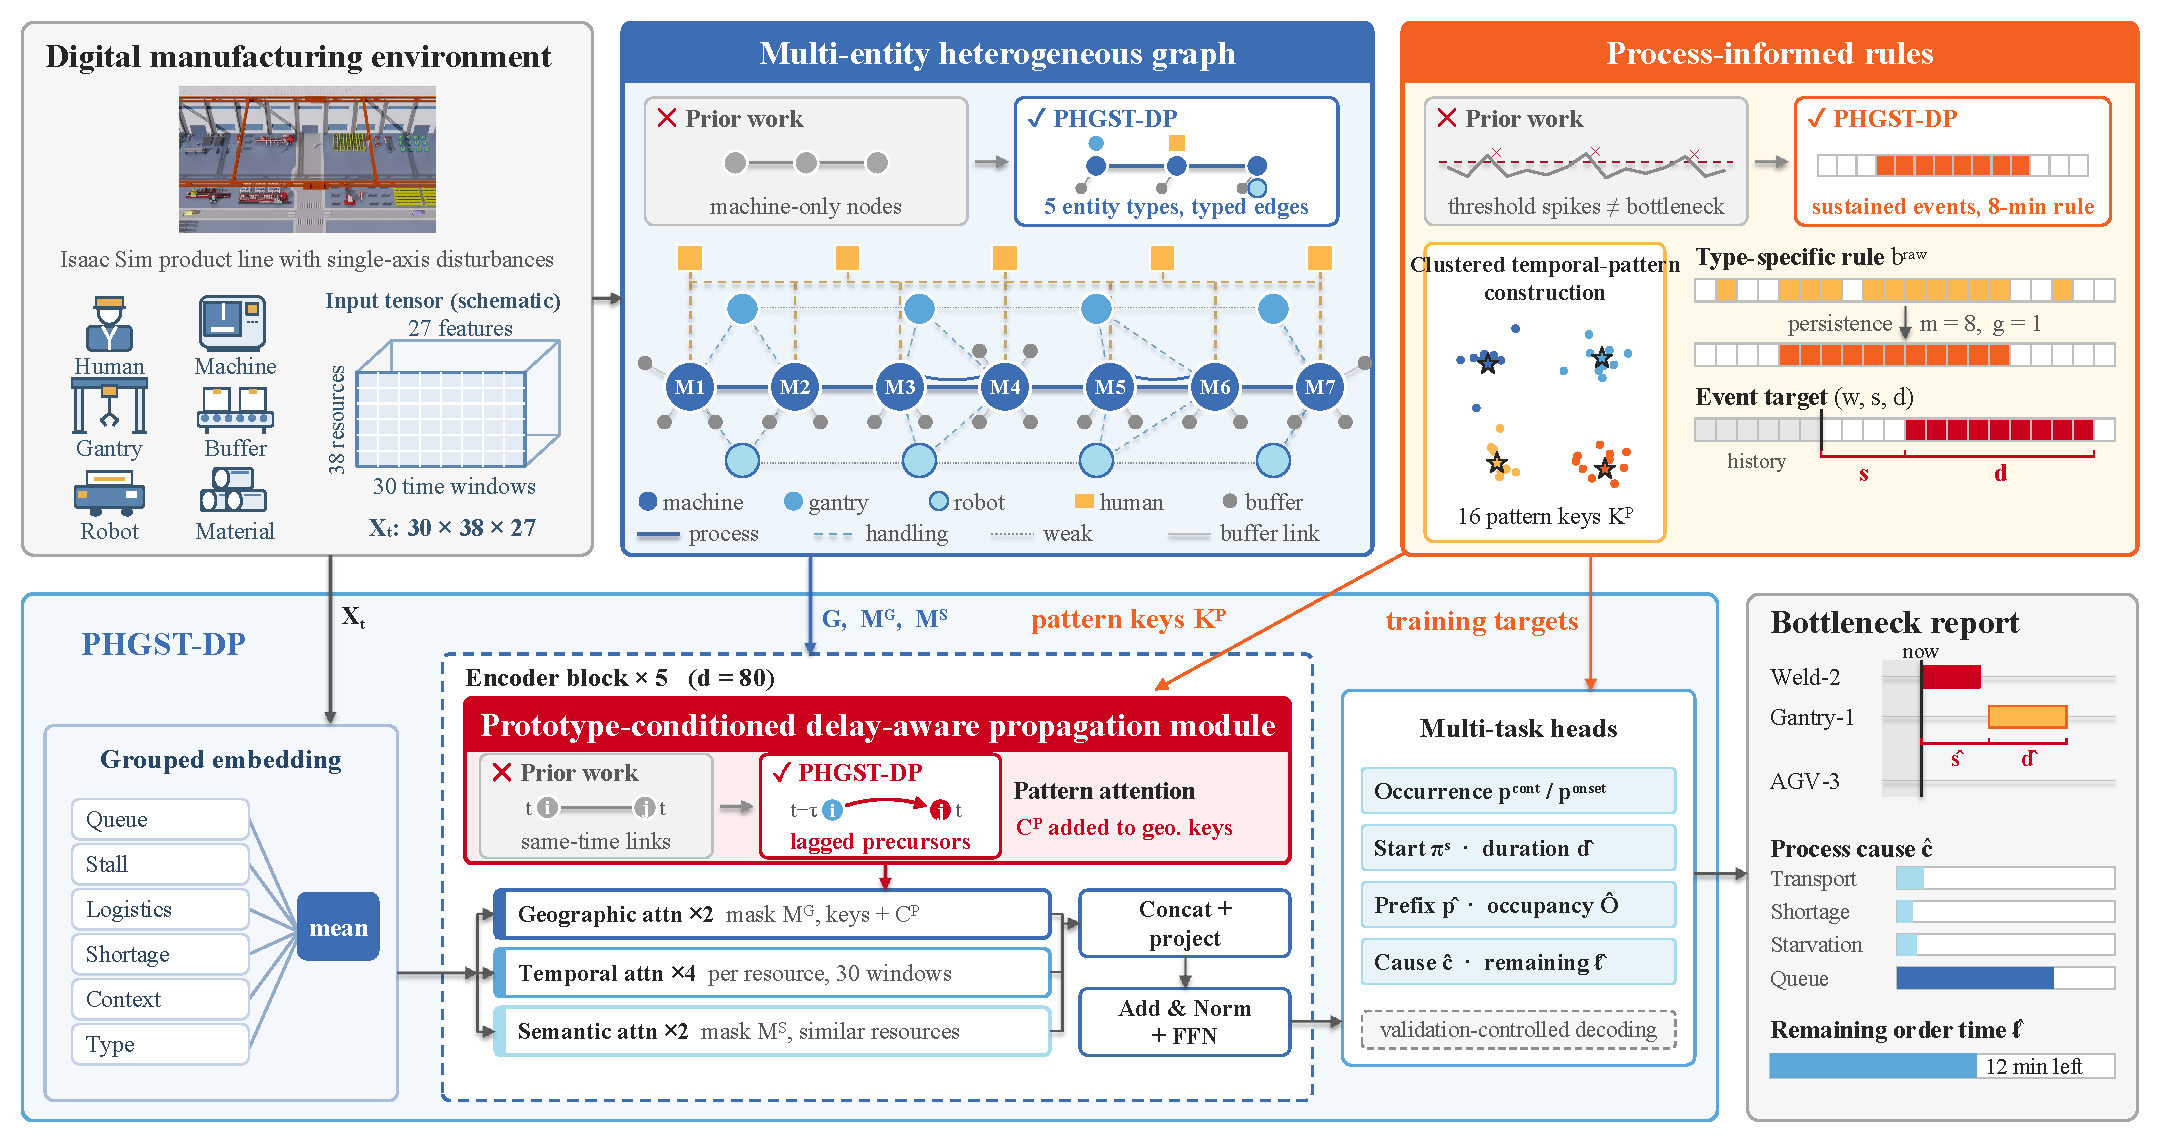
\includegraphics[width=\textwidth]{../figures/fig_method_final.pdf}
\caption{Overview of the problem formulation and the PHGST-DP method. Disturbance-controlled multi-entity observations, the heterogeneous factory graph, and process-informed event labels define the prediction problem. Grouped embedding, delay-pattern conditioning, and multi-task heads then produce the station-level bottleneck report.}
\label{fig:method-framework}
\end{figure*}

\subsection{Production system and resource relations}

The production system is defined through heterogeneous resource entities and typed process--logistics relations. This representation distinguishes the resources that receive bottleneck-event supervision from the contextual resources that influence how constraints form and propagate.


\subsubsection{Production task and resource entities}

We consider a shared digital-manufacturing line that produces water pipes through cutting, grooving, spot welding, root welding, surface welding, and finishing operations. The process is coupled with storage, gantry handling, transport-robot delivery, and human service. The graph implementation represents the primary process backbone with seven workstation nodes because parallel workbench and rotary-welding resources are retained as separate stations. Each production episode contains one order of ten products, and the nominal controller admits at most five products as concurrent WIP. It coordinates admission, process precedence, resource availability, and handling tasks; bottleneck prediction observes this controlled process but does not replace the controller.


Let the complete resource set be
\begin{equation}
\mathcal{R}=\mathcal{R}^{m}\cup\mathcal{R}^{g}\cup
\mathcal{R}^{a}\cup\mathcal{R}^{h}\cup\mathcal{R}^{b},
\end{equation}
where the superscripts denote machines and workbenches, gantries, transport robots, humans, and buffers. The retained graph contains 38 nodes: 7 machine/workbench nodes, 4 gantries, 4 transport robots, 5 humans, and 18 buffers. Material is not represented as a separate graph node; its state enters through shortage propagation, inbound waiting, affiliated-buffer occupancy, and other material-flow channels attached to the affected resources. These entities have different operational meanings. A machine transforms a product, a gantry or transport robot moves a product between locations, a human provides labour-dependent service, and a buffer stores intermediate products. The event-supervised target set is
\begin{equation}
\mathcal{S}=\mathcal{R}^{m}\cup\mathcal{R}^{g}\cup\mathcal{R}^{a}.
\end{equation}
Human and buffer nodes remain in the observation graph because labour availability and storage occupancy influence other resources, but the current implementation does not assign them station-event targets.


\subsubsection{Heterogeneous process--logistics graph}

The production system is represented as a weighted undirected graph
\begin{equation}
G=(\mathcal{R},E,A),\qquad
E=E^{p}\cup E^{f}\cup E^{b}\cup E^{l}\cup E^{w},
\end{equation}
where $E^{p}$ follows the seven-station process chain, $E^{f}$ connects parallel workstations belonging to the same equipment family, $E^{b}$ links storage buffers to affiliated machines, $E^{l}$ links handling agents to machine resources, and $E^{w}$ provides weak links among gantries or among transport robots. The implemented edge weights are $1.0$, $0.8$, $0.6$, $0.5$, and $0.3$ for these five relation groups, respectively, and every node receives a self-loop of weight $1.0$.


The graph is not intended to make the resources homogeneous. Instead, it specifies possible channels through which material flow, service delay, and congestion can propagate. Process edges encode downstream dependency; buffer edges expose storage-mediated blockage or starvation; and logistics edges connect a delayed machine input to the handling resources that can cause it. This distinction is important because two nodes may be structurally close but have different feature semantics, while two structurally distant nodes may exhibit similar operating trajectories. Section~\ref{sec:method} therefore derives both geographic and semantic attention masks from $G$ and the training trajectories.


\subsection{State representation and prediction targets}

The resource graph is observed through fixed production windows and paired with process-informed event and auxiliary targets. The following definitions align the historical input, future bottleneck interval, process cause, and order-level progress within one prediction sample.


\subsubsection{Windowed production state}

Raw simulation events are sampled at logical-second resolution and aggregated into non-overlapping windows of $\Delta=60$\,s. For resource $n$ and window $t$, the state $x_{t,n}\in\mathbb{R}^{27}$ contains twenty-one operational variables, five resource-type indicators, and one labour-saturation context variable. The operational variables cover queue and occupancy, activity and waiting, blockage and starvation, downtime, inter-departure variability, upstream/downstream interaction, route and inbound delay, shortage propagation, affiliated-buffer occupancy, disturbance context, and two turning-point/momentary indicators. Labour saturation is computed from the human states and broadcast only to machine nodes. The bottleneck score used by the offline aggregation pipeline is deliberately excluded from $x_{t,n}$ to avoid leaking a supervision signal into the predictor.


\begin{table}[t]
\centering
\caption{Semantic groups of the 27-dimensional resource state.}
\label{tab:feature-groups}
\scriptsize
\setlength{\tabcolsep}{3pt}
\renewcommand{\arraystretch}{1.12}
\begin{tabularx}{\columnwidth}{@{}l c >{\raggedright\arraybackslash}X@{}}
\toprule
Group & Dim. & Representative information \\
\midrule
Queue & 4 & Queue length, waiting, occupancy, growth \\
Stall & 6 & Blocked/starved time, stop, availability, coupling \\
Logistics & 4 & Departure variation, route/inbound delay, buffer \\
Shortage & 1 & Material-shortage propagation \\
Context & 7 & Activity, duration, time gap, disturbance, turning state, labour \\
Type & 5 & Machine, gantry, human, robot, buffer \\
\bottomrule
\end{tabularx}
\end{table}

Given $T_{\mathrm{in}}=30$ historical windows over $N$ resources, the model input is
\begin{equation}
X_t=\left[x_{\tau,n}\right]_
{\substack{\tau=t-T_{\mathrm{in}},\ldots,t-1\\n=1,\ldots,N}}
\in\mathbb{R}^{T_{\mathrm{in}}\times N\times 27}.
\end{equation}
The future label grid contains $H_{\mathrm{label}}=20$ one-minute windows. Within this grid, the admissible event onset $H_{\mathrm{start}}$ is varied between experimental settings. Separating the label grid from the onset cap allows an event to begin within the warning range while retaining enough future windows to represent its persistence.


\subsubsection{Process-informed bottleneck-event construction}

A bottleneck label must distinguish a production-relevant constraint from ordinary activity or travel. For each supervised resource, the implementation first applies a type-dependent rule
\begin{equation}
b^{\mathrm{raw}}_{t,n}=\Phi_{\rho(n)}(x_{t,n},X_t)\in\{0,1\},
\end{equation}
where $\rho(n)$ is the resource type. For a machine, $\Phi_m$ combines queue accumulation with blocked or starved time, coupled upstream/downstream evidence, shortage propagation, inbound or route delay, downtime, and labour-related waiting. A disturbance flag alone is insufficient: it must coincide with queue, stall, or unavailability evidence. For a gantry, a hot state requires route or inbound delay with stalling, or a stop/unavailable state. For a transport robot, inbound waiting must coincide with stalling, or the robot must be frozen/stopped; normal route travel is not considered a bottleneck.


The raw binary grid is converted into sustained occupancy. In the retained configuration, runs shorter than $m=8$ windows are removed first; an internal cold gap of at most $g=1$ window is then filled when it lies between retained hot regions. Denoting short-run removal by $\mathcal{D}_{m}$ and gap filling by $\mathcal{F}_{g}$, the implemented legacy order is
\begin{equation}
o_{:,n}=\mathcal{F}_{g}\!\left(\mathcal{D}_{m}
\left(b^{\mathrm{raw}}_{:,n}\right)\right).
\end{equation}
This persistence requirement rejects isolated threshold crossings. It should not be confused with the offline event CSV, whose score-event merge can retain a one-window event; PHGST-DP training targets are generated from the operational occupancy grid and use the eight-window criterion.


For a history ending immediately before window $t$, the primary target for station $n$ is
\begin{equation}
y_{t,n}^{\mathrm{evt}}=(w_{t,n},s_{t,n},d_{t,n}),
\end{equation}
where $w_{t,n}$ indicates that an eligible run exists, $s_{t,n}$ is its onset offset, and $d_{t,n}$ is its length within the future grid. If the resource is hot in the final history window and the future run begins at offset zero, the event is \emph{ongoing}; its future remainder may be shorter than eight windows because the full event already satisfied persistence before the observation boundary. Otherwise, a run with $s_{t,n}>0$ is \emph{upcoming} and must satisfy the configured minimum duration. If several runs are available for one station, the longest eligible run is selected rather than the earliest run.


Algorithm~\ref{alg:event} states this construction in the order used to build the training targets. Human and buffer nodes are omitted because they are not in $\mathcal{S}$.


\begin{algorithm}[t]
\caption{Bottleneck-event construction.}
\label{alg:event}
\KwIn{$\{x_{t,n}\}$; type $\rho$; $m{=}8$; $g{=}1$; cap $H_{\mathrm{start}}$}
\KwOut{$o_{:,n}$ and $(w_{t,n},s_{t,n},d_{t,n})$}
\tcp*[f]{Step 1: type-dependent raw state}\;
\ForEach{$n\in\mathcal{S}$ and window $t$}{
  $b^{\mathrm{raw}}_{t,n}\leftarrow\Phi_{\rho(n)}(x_{t,n})$\;
}
\tcp*[f]{Step 2: drop short runs, then fill gaps}\;
\ForEach{$n\in\mathcal{S}$}{
  drop hot runs shorter than $m$\;
  fill a cold gap of length at most $g$\;
  $o_{:,n}\leftarrow\mathcal{F}_{g}(\mathcal{D}_{m}(b^{\mathrm{raw}}_{:,n}))$\;
}
\tcp*[f]{Step 3: longest run inside the cap}\;
\ForEach{$n\in\mathcal{S}$ at history end $t$}{
  $(s,d)\leftarrow$ longest future hot run\;
  \eIf{history ends hot and $s=0$}{
    $(w_{t,n},s_{t,n},d_{t,n})\leftarrow(1,s,d)$ \tcp*{ongoing}
  }{
    \eIf{$d\ge m$ and $0<s\le H_{\mathrm{start}}$}{
      $(w_{t,n},s_{t,n},d_{t,n})\leftarrow(1,s,d)$ \tcp*{upcoming}
    }{
      $w_{t,n}\leftarrow 0$\;
    }
  }
}
\end{algorithm}

\subsubsection{Cause and order-level targets}

Station events identify where and when production is constrained, but intervention also requires a process explanation. The aggregation pipeline assigns a window-level cause through a fixed evidence priority: material shortage, transport delay, queue buildup, downstream blockage, upstream starvation, and high utilization. The label is inferred from measured shortage, inbound/route delay, queue, blocked, starved, and activity variables; it is not copied from the injected disturbance dimension. This permits, for example, a machine disturbance to create a downstream starvation label after propagation.


The reported cause set is
\begin{equation}
\begin{aligned}
\mathcal{C}=\{&
\text{transport delay},\text{material shortage},\\
&\text{upstream starvation},\text{queue buildup}\}.
\end{aligned}
\end{equation}
Other configured cause indices are ignored by the loss because they lack sufficient train/test support. The order-level target $\ell_t$ is the number of future one-minute windows until all jobs are complete under the configured prediction cap. It provides a line-level estimate of production consequence that complements the station-level event report.


Algorithm~\ref{alg:cause} applies the priority to one hot window. A label outside $\mathcal{C}$ is stored but receives zero weight in the cause loss.


\begin{algorithm}[t]
\caption{Cause assignment.}
\label{alg:cause}
\KwIn{shortage, delay, queue, wait, buffer, blockage, starvation, activity}
\KwOut{cause label and its loss weight}
\If{shortage exceeds its threshold}{
  \Return material shortage, weight $1$\;
}
\If{inbound or route delay is high}{
  \Return transport delay, weight $1$\;
}
\If{queue, wait, or buffer shows buildup}{
  \Return queue buildup, weight $1$\;
}
\If{blockage exceeds starvation}{
  \Return downstream blockage, weight $0$\;
}
\If{starvation is positive}{
  \Return upstream starvation, weight $1$\;
}
\If{activity fraction is high}{
  \Return high utilization, weight $0$\;
}
\Return residual label, weight $0$\;
\end{algorithm}

\subsection{Multi-task prediction formulation}

The complete prediction problem is the mapping
\begin{equation}
f_{\theta}:(X_t,G)\longmapsto
\left(
\{\hat w_{t,n},\hat s_{t,n},\hat d_{t,n}\}_{n\in\mathcal{S}},
\hat c_t,\hat\ell_t
\right).
\end{equation}
This formulation differs from forecasting a bottleneck score. The output specifies the affected resource, event onset, persistence, process explanation, and expected order impact in a common decision-oriented interface. The method in Section~\ref{sec:method} parameterizes $f_{\theta}$ with a delay-aware heterogeneous spatiotemporal encoder and multiple task heads.


The delayed-propagation challenge is contained in this mapping rather than introduced as an additional label. For an upcoming event at target resource $j$, predictive evidence may occur at another resource $i$ and at an earlier history offset $\tau$. The model must therefore learn associations of the form
\begin{equation}
(x_{t-\tau,i},\,i\!\rightarrow\!j)\longmapsto y^{\mathrm{evt}}_{t,j},
\qquad \tau>0,
\end{equation}
where $i\!\rightarrow\!j$ denotes a possible process or logistics route, not a proven physical causal path. This formulation motivates conditioning cross-resource interaction on recurrent historical patterns while evaluating success only through the future event report.


Two event criteria are distinguished. A station-level hit requires that the predicted resource equal the labelled resource. A stricter report-level true positive additionally requires
\begin{equation}
|\hat{s}_{t,n}-s_{t,n}|\leq\epsilon_s,\qquad
\epsilon_s=3~\mathrm{min}.
\end{equation}
Occurrence precision, recall, and F1 quantify the coverage and reliability of alarms. Start, duration, and remaining-time errors are conditional or regression measures and cannot compensate for a missed station event. Ongoing and upcoming recalls are therefore reported separately: the latter is the direct measure of whether the model provides warning before the bottleneck becomes visible at the target station.


%% ========================================================================
\section{Methodology} \label{sec:method}
%% ========================================================================

\subsection{Method overview}

PHGST-DP is organized around the three contributions established in Section~\ref{sec:intro}. First, controlled simulation, a heterogeneous factory graph, and grouped embedding integrate machine, human, material-flow, buffer, gantry, and transport evidence. Second, process-informed event construction and recurrent-pattern grouping address scarce, weakly separable supervision while retaining traceability to observable production evidence. Third, pattern-enhanced spatiotemporal attention addresses delayed propagation. The complete information flow is
\begin{equation}
\begin{aligned}
\text{simulation}&\rightarrow\text{window/event construction}\\
&\rightarrow\text{factory graph}\rightarrow\text{joint prediction}.
\end{aligned}
\end{equation}
The first two stages create reproducible observations and targets. The latter two parameterize the mapping $f_\theta$ defined in Section~\ref{sec:problem}.


Figure~\ref{fig:model-architecture} presents the PHGST-DP model architecture. The multi-entity history is partitioned into six semantic feature groups and combined with temporal, graph-Laplacian, and node-identity embeddings. Each encoder block separates temporal, geographic, and semantic dependencies; short-pattern prototypes condition the geographic keys so that recurrent precursors can influence cross-resource interaction after a delay. Station-level and graph-level heads then decode occurrence, onset, duration, future occupancy, process cause, and remaining order time.


\begin{figure*}[t]
\centering
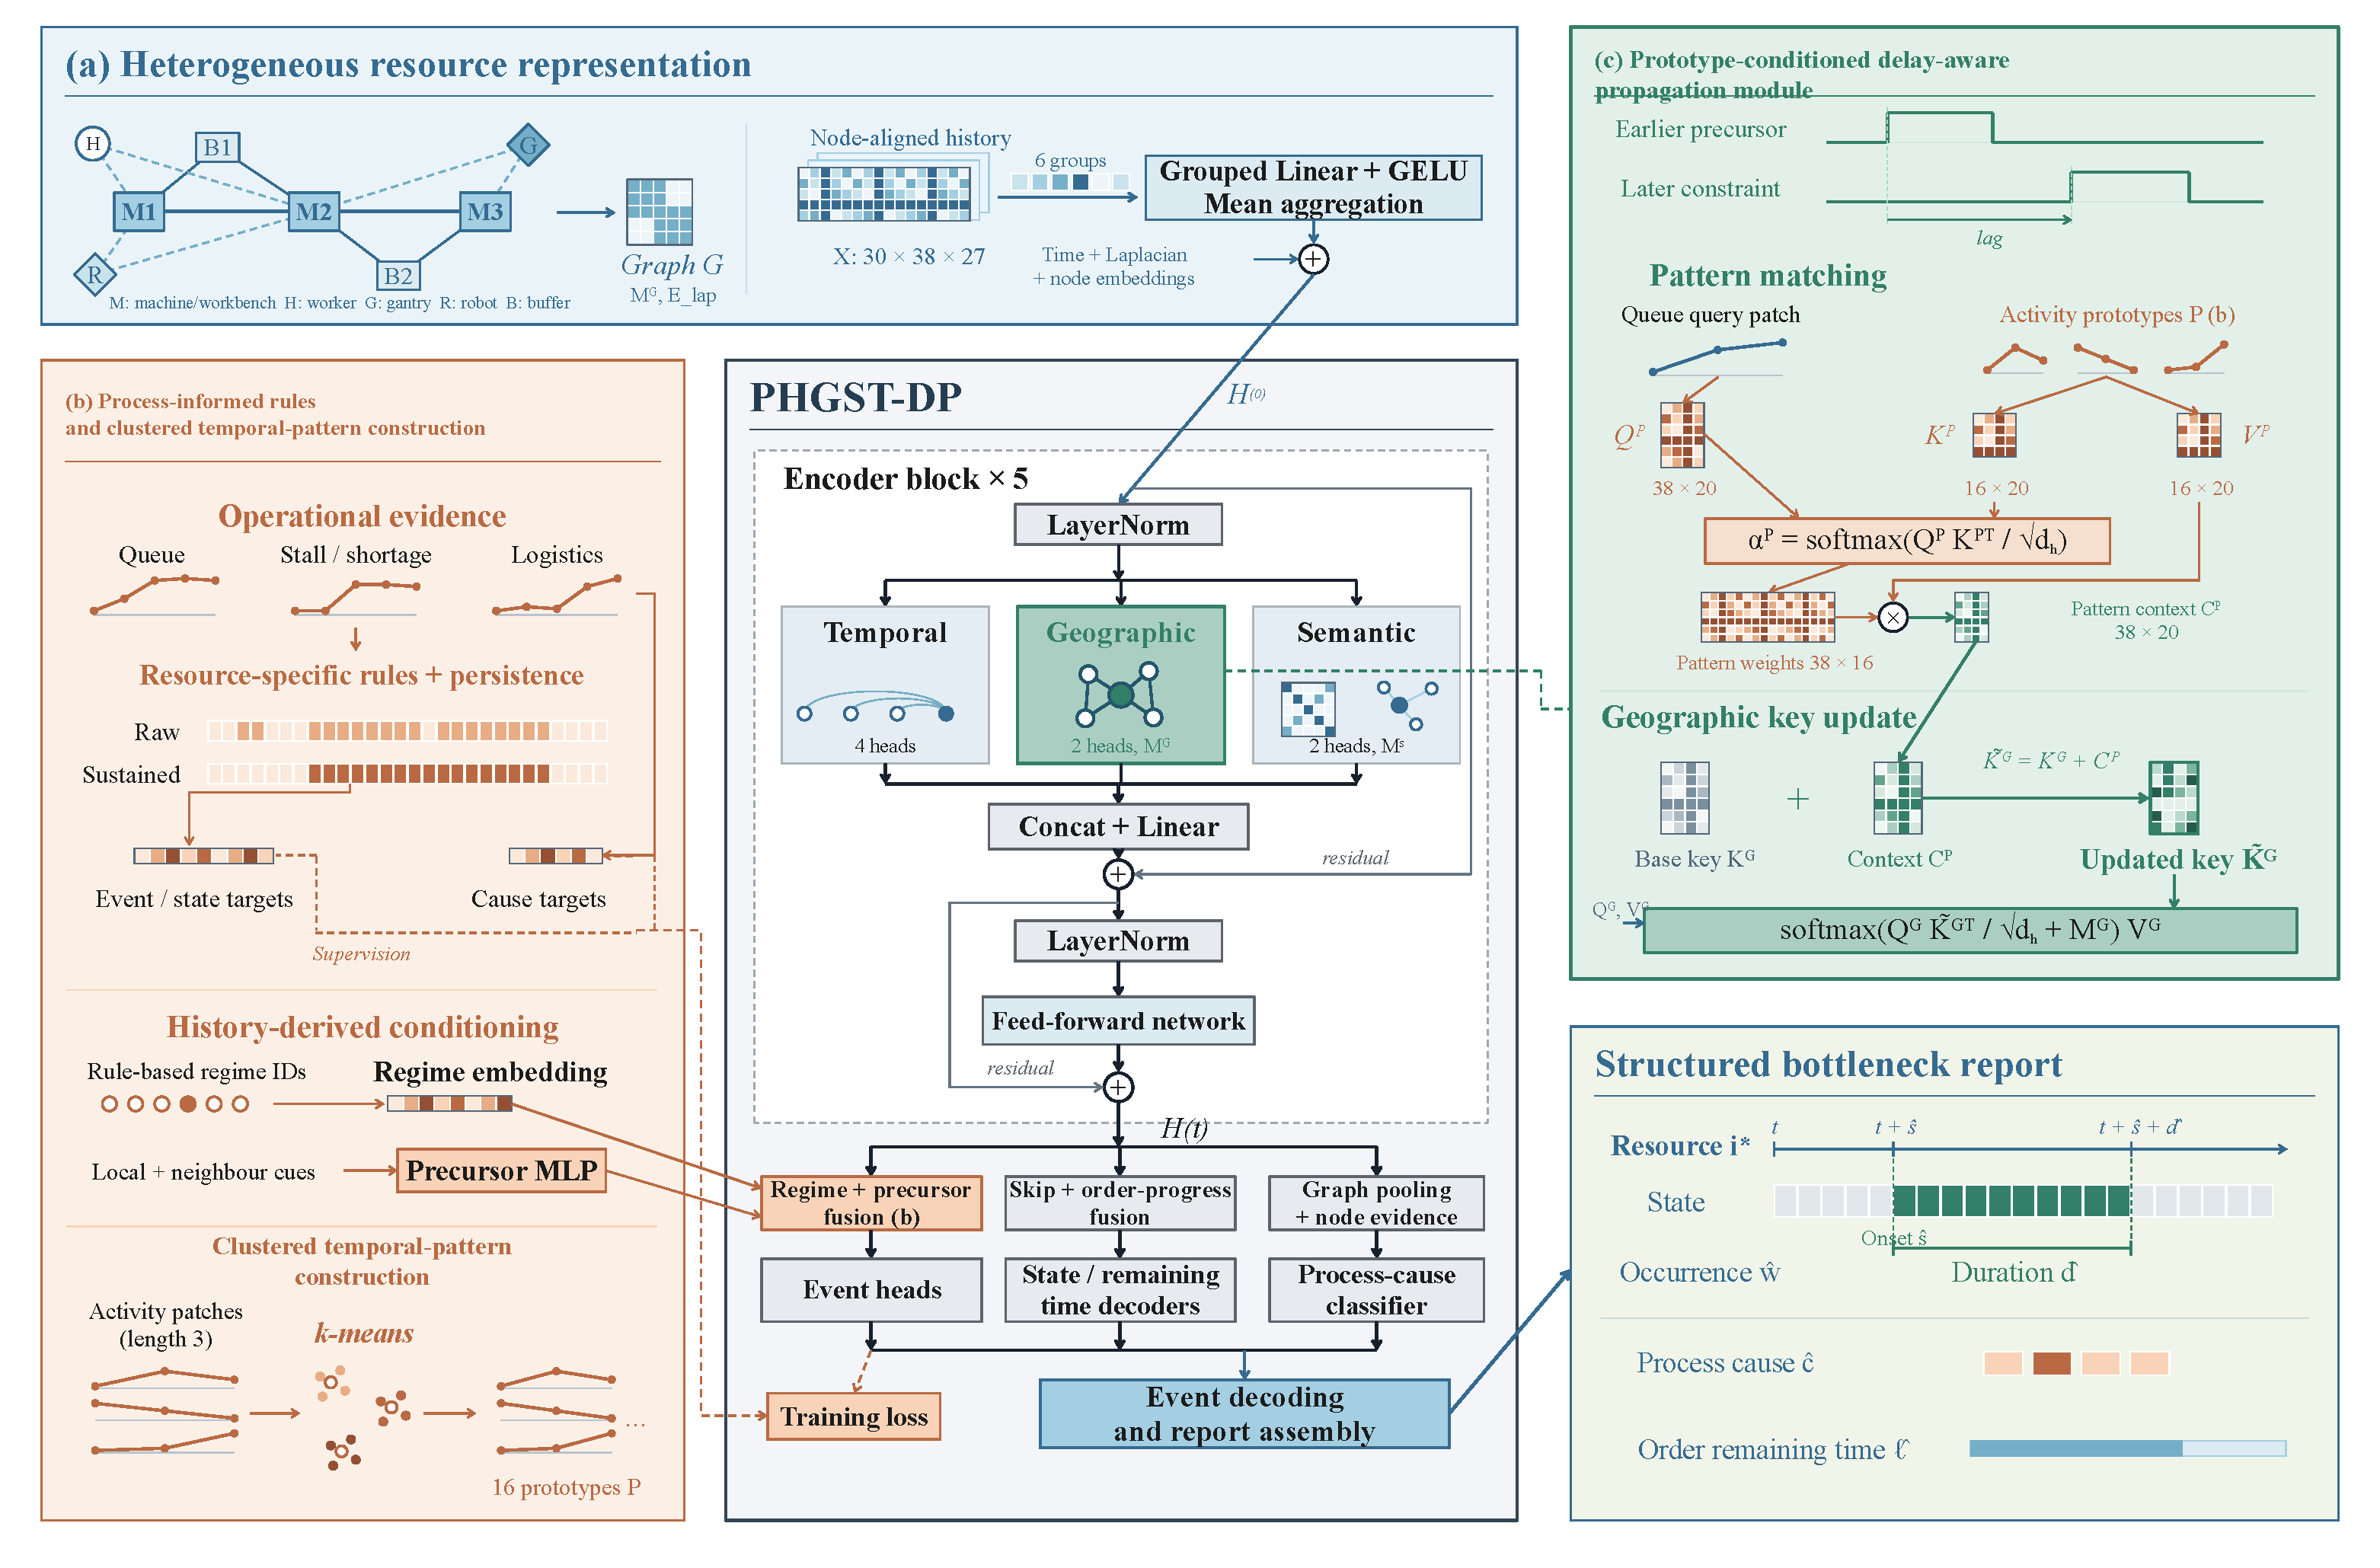
\includegraphics[width=\textwidth]{../figures/fig_model_final.pdf}
\caption{Architecture of PHGST-DP. Grouped heterogeneous embeddings combine the multi-entity history with temporal, structural, and node-identity context. Five encoder blocks model temporal, geographic, and semantic dependencies, while pattern attention injects recurrent short-pattern context into geographic keys for delay-aware cross-resource interaction. Multi-task heads produce station-level event attributes and graph-level process explanations.}
\label{fig:model-architecture}
\end{figure*}

Algorithm~\ref{alg:phgst-train} is the outer loop around that architecture. Labels, masks, and pattern centres are fixed before the parameter update. Test episodes are read only after Algorithm~\ref{alg:decode} freezes the checkpoint and threshold.


\begin{algorithm}[t]
\caption{Training and held-out evaluation.}
\label{alg:phgst-train}
\KwIn{episodes; graph $G$; $T_{\mathrm{in}}$; $H_{\mathrm{label}}$}
\KwOut{frozen $\theta^{\star}$ and threshold $\tau^{\star}$}
\tcp*[f]{Labels and graph, fixed first}\;
Aggregate each episode into $60$\,s windows\;
Run Algorithms~\ref{alg:event} and~\ref{alg:cause}\;
Build $A$, $M^{G}$, $M^{S}$, and Laplacian positions\;
Fit $16$ centres on length-$3$ activity patches\;
\tcp*[f]{Parameter update}\;
\For{each epoch}{
  \For{each in-episode minibatch}{
    evaluate Algorithm~\ref{alg:forward}\;
    take one gradient step on $\mathcal{L}$\;
  }
  update the validation choice with Algorithm~\ref{alg:decode}\;
}
Freeze $\theta^{\star}$ and $\tau^{\star}$\;
Evaluate the held-out episodes once\;
\end{algorithm}

\subsection{Multi-entity data and graph construction}

This stage constructs the synchronized resource--time tensor, process-consistent supervision, and graph constraints used by PHGST-DP. It proceeds from traceable disturbance-controlled trajectories to aligned multi-entity states and then to the structural and semantic masks required by the encoder.


\subsubsection{Disturbance-controlled digital production line}

The data-generation environment reconstructs the water-pipe line, resource layout, storage locations, and handling activities in NVIDIA Isaac Sim. At every logical second, the collector records the episode configuration, active disturbance, resource-state transitions, job traces, buffer events, transport tasks, and material inventory. These streams are synchronized by episode and logical time, allowing a downstream event to be traced back through the states that preceded it. Only episodes in which all ten products complete are exported, and episodes containing a deadlock reset are removed.


Formal single-axis collection activates one disturbance dimension at intensity $I=1.0$ while leaving the other dimensions nominal:
\begin{itemize}
 \item[$\bullet$] \textbf{Machine disturbance} increases processing-time variation, lowers successful operation probability, disables selected workstations, and inserts temporary machine-fault pulses.
 \item[$\bullet$] \textbf{Human disturbance} reduces the workforce from five to three, increases task-time variation, and inserts temporary leave periods.
 \item[$\bullet$] \textbf{Logistics disturbance} reduces transport robots from four to two, slows gantry motion, and inserts handling freezes that include an AGV freeze.
 \item[$\bullet$] \textbf{Material disturbance} temporarily hides flange or elbow kits and introduces additional shortage pulses for selected stock-keeping units.
\end{itemize}
The temporary machine, human, and logistics pulses last at least ten logical minutes. This design does not assume that the injected dimension is the final bottleneck cause. Its purpose is to produce traceable perturbations whose operational consequences can emerge at different resources and times.


Mixed two-, three-, and four-dimension episodes are exported as a separate dataset. They are not merged into the retained single-axis dataset because simultaneous shocks change both event prevalence and the attribution problem. This separation permits the main model to be trained on interpretable perturbation trajectories and allows mixed disturbances to be examined later as a distribution-expansion experiment.


\subsubsection{Multi-entity aggregation and process-consistent supervision}

The second stage converts heterogeneous raw logs into a common resource--time grid. Statistics are aggregated over non-overlapping one-minute windows and aligned by resource identifier. Missing resource states are completed through the export pipeline, type one-hot variables are appended, and labour saturation is recomputed from the available human nodes. The resulting tensor contains 38 resource nodes and 27 channels in the retained dataset. Episode boundaries are preserved throughout sliding-window generation, preventing a history from combining observations from two production runs.


Event supervision follows the type-specific occupancy and persistence definitions in Section~\ref{sec:problem}. The retained configuration uses operational-state targets rather than the exported bottleneck-score column. Consequently, the model cannot solve the task by reproducing the score used during aggregation. The event target builder scans each station's future occupancy, rejects ineligible upcoming runs, preserves the short remainder of an already established ongoing event, applies the configured onset cap, and selects the longest eligible run. This produces mutually aligned occurrence, onset, duration, occupancy-grid, and prefix targets.


Three different clustering-related objects are kept conceptually separate. First, the offline aggregation tools can produce station- and window-level $K=8$ k-means descriptors for exploratory regime analysis. Second, the training dataset derives cause-aligned regime identifiers by deterministic rules and can use them for representation conditioning and contrastive regularization. Third, short temporal patches are clustered to create the pattern keys used by geographic attention. Only the third object is an active clustering mechanism in the retained delay module. The offline cluster-prediction loss has weight zero, and no cluster index defines the bottleneck ground truth; event labels are produced only by the process rules and persistence filter above.


\subsubsection{Heterogeneous factory graph and attention masks}

The weighted adjacency $A$ follows the relation definitions in Section~\ref{sec:problem}. Floyd--Warshall shortest-path computation converts nonzero edges into hop distances $D^{\mathrm{hop}}$. The geographic mask is
\begin{equation}
M^G_{ij}=
\begin{cases}
0, & D^{\mathrm{hop}}_{ij}<\delta_G,\\
-\infty, & \text{otherwise},
\end{cases}
\qquad \delta_G=4,
\end{equation}
so a node attends only to resources fewer than four hops away in geographic attention. This mask allows information to cross more than one process or logistics edge while excluding globally unrelated nodes.


Geographic proximity alone cannot capture parallel or substitutable resources with similar behaviour. A semantic distance matrix is therefore computed from training trajectories. The feature channels of each node are first averaged to form a scalar trajectory $\bar x_{:,i}$, after which
\begin{equation}
D^{\mathrm{sem}}_{ij}
=1-\mathrm{corr}(\bar{x}_{:,i},\bar{x}_{:,j}).
\end{equation}
For each node, the five nearest trajectories are unmasked in $M^S$; all others are suppressed. This implementation uses Pearson correlation distance as a short-episode substitute for the dynamic-time-warping distance used in traffic PDFormer. Finally, the nontrivial eigenvectors of the normalized graph Laplacian provide an eight-dimensional structural position for every resource.


\subsection{Delay-aware heterogeneous spatiotemporal encoding}

The encoder first preserves the distinct semantics of heterogeneous observations through grouped embedding and then models temporal evolution, graph propagation, and behavioural similarity. Delay-pattern conditioning further links current resource states with recurrent precursor patterns whose effects emerge later in the production process.


\subsubsection{Grouped heterogeneous state embedding}

Directly projecting all 27 channels with one linear layer would treat queue length, downtime, type codes, and shortage evidence as if they shared one measurement semantics. The grouped token embedding instead partitions the channels into queue, stall, logistics, shortage, context, and type groups. Each group $q$ has an independent affine projection and GELU activation:
\begin{equation}
e^{(q)}_{t,n}=\mathrm{GELU}
\left(W_q x^{(q)}_{t,n}+b_q\right).
\end{equation}
The six group embeddings are mean-pooled, rather than concatenated as separate tokens:
\begin{equation}
e_{t,n}=\frac{1}{6}\sum_{q=1}^{6}e^{(q)}_{t,n}.
\end{equation}
This operation places heterogeneous evidence in a common latent space while preventing a high-dimensional group from dominating solely through channel count.


The initial representation combines grouped evidence with temporal, structural, and identity information:
\begin{equation}
H^{(0)}=E_{\mathrm{group}}(X_t)+
E_{\mathrm{time}}+E_{\mathrm{lap}}(G)+E_{\mathrm{node}}.
\end{equation}
$E_{\mathrm{time}}$ is sinusoidal, $E_{\mathrm{lap}}$ projects the graph eigenvectors, and $E_{\mathrm{node}}$ is a learned resource-identity embedding. Day-of-week and time-of-day embeddings are disabled because an episode is driven by order progress and disturbances rather than calendar periodicity.


\subsubsection{Pattern-conditioned spatiotemporal encoder}

The encoder must distinguish three dependencies: evolution of one resource through time, propagation through the process--logistics graph, and similarity between resources that need not be adjacent. Each encoder block therefore allocates separate attention heads to temporal, geographic, and semantic attention. For an attention branch $b\in\{T,G,S\}$,
\begin{equation}
\mathrm{Attn}_{b}(Q_b,K_b,V_b;M_b)
=\mathrm{softmax}\!\left(
\frac{Q_bK_b^\top}{\sqrt{d_h}}+M_b
\right)V_b ,
\end{equation}
where temporal attention has no cross-node mask, geographic attention uses $M^G$, and semantic attention uses $M^S$.


Delayed propagation is introduced through data-derived short-pattern keys. In the retained implementation, the prototype bank is fitted by applying k-means with sixteen centres to length-three patches of the configured activity channel (\texttt{active\_pct\_s}), whereas online query patches use the first model-output channel (\texttt{queue\_length\_s}). Let $P_{t,n}$ denote a queue query patch and $K^P$ the learned activity-pattern centres. Pattern attention computes
\begin{equation}
C^P_{t,n}=
\mathrm{softmax}\!\left(
\frac{Q^P(P_{t,n})K^P(K^P)^\top}{\sqrt{d_h}}
\right)V^P(K^P).
\end{equation}
The resulting cross-channel pattern context is added to the geographic key before geographic attention is evaluated. Thus, spatial interaction is conditioned not only on node proximity but also on the learned association between current queue evolution and recurrent activity prototypes. The mechanism does not use a Fourier transform.


For encoder block $l$, the three branches are
\begin{equation}
\begin{aligned}
H_T^{(l)}&=\mathrm{Attn}_T(H^{(l-1)}),\\
H_G^{(l)}&=\mathrm{Attn}_G(H^{(l-1)},M^G,C^P),\\
H_S^{(l)}&=\mathrm{Attn}_S(H^{(l-1)},M^S).
\end{aligned}
\end{equation}
Their outputs are concatenated, projected, and processed by pre-normalized residual and feed-forward layers. The retained configuration uses five blocks with latent dimension 80. It allocates four temporal heads, two geographic heads, and two semantic heads; these are separate branches rather than one undifferentiated eight-head attention module.


\subsection{Multi-task bottleneck prediction and optimization}

The shared spatiotemporal representation is converted into station-level event reports and graph-level explanatory outputs. The prediction heads, joint objective, and validation-controlled decoder form a single sequence from latent representation to the final operational report.


\subsubsection{Event, occupancy, and explanatory heads}

Let $z_{t,n}$ be the final representation of supervised station $n$. The event occurrence module contains separate logits for continuation and future onset:
\begin{equation}
p^{\mathrm{cont}}_{t,n}=\sigma(f_{\mathrm{cont}}(z_{t,n})),
\qquad
p^{\mathrm{onset}}_{t,n}=\sigma(f_{\mathrm{onset}}(z_{t,n})).
\end{equation}
The history-end occupancy selects which logit is used for the combined occurrence probability. This split prevents the abundant ongoing pattern from dominating the weaker precursor pattern of an upcoming event. A start head produces a categorical distribution over future minute offsets, while duration and prefix heads produce nonnegative lengths:
\begin{equation}
\begin{aligned}
\pi^s_{t,n}&=\mathrm{softmax}(f_s(z_{t,n})),\\
\hat d_{t,n}&=\mathrm{softplus}(f_d(z_{t,n})),\\
\hat p_{t,n}&=\mathrm{softplus}(f_p(z_{t,n})).
\end{aligned}
\end{equation}


An occupancy decoder predicts the complete future hot grid $\hat O_t\in[0,1]^{H_{\mathrm{label}}\times N}$. It acts as dense temporal supervision for the sparse event tuple. The prefix prediction estimates how long a hot segment continues from the first future window and is used to distinguish a truly continuing bottleneck from a station that was hot at the end of history but immediately recovers. A precursor branch additionally combines local queue/stall evidence with neighbourhood information before occurrence prediction.


Order remaining time and cause are graph-level outputs. The final node states are pooled through mean aggregation and a maximum gated-node score, then concatenated with order-progress information:
\begin{equation}
\begin{aligned}
u_t&=\mathrm{AuxPool}(H_t^{(L)},\text{order state}),\\
\hat\ell_t&=f_\ell(u_t),\qquad \hat c_t=f_c(u_t).
\end{aligned}
\end{equation}
The cause head retains ten output indices for checkpoint compatibility, but training and inference are restricted to the four supported report classes. This preserves implementation compatibility without presenting unsupported classes as evaluated predictions.


Algorithm~\ref{alg:forward} assembles these stages into one evaluation of $f_{\theta}$. Pattern centres condition geographic keys inside every block; they are not recomputed from the current minibatch.


\begin{algorithm}[t]
\caption{Delay-pattern forward pass.}
\label{alg:forward}
\KwIn{$X_t$; masks $M^{G},M^{S}$; centres $K^{P}$}
\KwOut{events, occupancy $\hat O_t$, cause $\hat c_t$, time $\hat\ell_t$}
\tcp*[f]{Grouped embedding}\;
\ForEach{group $q$}{
  $e^{(q)}\leftarrow\mathrm{GELU}(W_q x^{(q)}+b_q)$\;
}
$H^{(0)}\leftarrow\mathrm{mean}_{q}e^{(q)}+E_{\mathrm{time}}+E_{\mathrm{lap}}+E_{\mathrm{node}}$\;
\tcp*[f]{Five pre-norm blocks}\;
\For{$l\leftarrow 1$ \KwTo $5$}{
  $H_T\leftarrow\mathrm{Attn}_{T}(H^{(l-1)})$\;
  match length-$3$ queue patches to $K^{P}$\;
  add that context to the geographic keys\;
  $H_G\leftarrow\mathrm{Attn}_{G}(H^{(l-1)},M^{G})$\;
  $H_S\leftarrow\mathrm{Attn}_{S}(H^{(l-1)},M^{S})$\;
  $H^{(l)}\leftarrow\mathrm{FFN}(\mathrm{Proj}[H_T;H_G;H_S])$\;
}
\tcp*[f]{Station and graph heads}\;
\ForEach{$n\in\mathcal{S}$}{
  \eIf{$n$ ends hot}{
    use the continuation logit\;
  }{
    use the onset logit\;
  }
  $\pi^{s}\leftarrow\mathrm{softmax}(f_s(z_n))$\;
  $\hat d\leftarrow\mathrm{softplus}(f_d(z_n))$\;
}
$\hat O_t\leftarrow\sigma(f_O(H^{(5)}))$\;
pool nodes and order progress for $\hat\ell_t$ and $\hat c_t$\;
\end{algorithm}

\subsubsection{Joint training objective}

The learning objective is organized into primary event terms, dense temporal terms, explanatory terms, and representation regularizers:
\begin{equation}
\begin{aligned}
\mathcal{L}={}&
\lambda_w\mathcal{L}_{\mathrm{will}}+
\lambda_{on}\mathcal{L}_{\mathrm{onset}}+
\lambda_s\mathcal{L}_{\mathrm{start}}+
\lambda_d\mathcal{L}_{\mathrm{dur}}\\
&+\lambda_p\mathcal{L}_{\mathrm{prefix}}+
\lambda_o\mathcal{L}_{\mathrm{occ}}+
\lambda_{\ell}\mathcal{L}_{\mathrm{remain}}+
\lambda_c\mathcal{L}_{\mathrm{cause}}\\
&+\lambda_r\mathcal{L}_{\mathrm{recon}}+
\lambda_q\mathcal{L}_{\mathrm{contrast}}+
\lambda_{\mathrm{tpm}}\mathcal{L}_{\mathrm{tpm}} .
\end{aligned}
\end{equation}
The occurrence loss combines reweighted binary cross-entropy, focal modulation, hard-false-positive weighting, and an internal differentiable F1 term. Separate onset supervision is applied to the cold-history head. The start loss uses a Gaussian soft target over minute offsets, whereas duration, prefix, and remaining time use log-transformed Smooth-L1 regression. Remaining-time samples are further weighted by order progress.


The occupancy term combines type-balanced binary cross-entropy, soft Dice, and soft intersection-over-union losses. Cause classification uses class-weighted cross-entropy only for supported hot-window labels. Future-feature reconstruction and graph-level supervised contrastive learning regularize the shared representation, while an auxiliary turning-point/momentary signal contributes a binary loss. In the retained configuration, legacy score, will, mark, time-to-start, STGNPP, and offline cluster-head losses are all disabled. In particular, $\lambda_{\mathrm{cluster}}=0$; the headline event prediction is not optimized to reproduce offline k-means assignments.


\subsubsection{Validation-controlled report decoding}

Training loss alone does not define an operational report. At inference, PHGST-DP first chooses the continuation logit for historically hot stations and the onset logit for historically cold stations. Prefix evidence can lift an ongoing occurrence and set its onset to zero. Predicted occupancy runs can be united with the event head when they satisfy the minimum-duration rule, including a separate upcoming union. Type-specific report thresholds are retained for gantries and transport robots, and events whose predicted onset exceeds the active cap are removed.


The global report threshold is not tuned on the test set. Candidate thresholds are swept on validation data. The retained checkpoint must satisfy the configured validation precision and recall gate when possible, after which station F1 determines selection; if no candidate opens the gate, the documented fallback rule is used. The chosen checkpoint and threshold are then frozen for held-out evaluation. This separation is essential because the decoder contains several event-consistency rules and could otherwise be inadvertently fitted to the test distribution.


Algorithm~\ref{alg:decode} is the corresponding report procedure. Candidate thresholds are compared on validation predictions only.


\begin{algorithm}[t]
\caption{Report decoding on validation.}
\label{alg:decode}
\KwIn{logits; prefix; occupancy $\hat O$; history-end state}
\KwOut{reported events and threshold $\tau^{\star}$}
\tcp*[f]{One supervised station}\;
\ForEach{$n\in\mathcal{S}$}{
  \eIf{$n$ ends hot}{
    use the continuation probability\;
    \If{the prefix run is long enough}{
      set the onset to $0$\;
    }
  }{
    use the onset probability\;
  }
  \If{$\hat O$ contains a sufficiently long run}{
    unite that run with the event head\;
  }
  apply the type threshold of $n$\;
  \If{the onset exceeds the active cap}{
    drop station $n$\;
  }
}
\tcp*[f]{Threshold sweep does not read the test set}\;
\ForEach{candidate $\tau$}{
  record precision, recall, and station F1\;
}
\eIf{a candidate passes both gates}{
  keep the checkpoint with the best station F1\;
}{
  keep the best ungated checkpoint\;
}
\end{algorithm}

%% ========================================================================
\section{Experiments}\label{sec:exp}

PHGST-DP is evaluated for a central production objective: identifying emerging bottlenecks with sufficient temporal and process detail to support intervention planning. The experiments connect event detection and early warning with duration and state prediction, then examine the heterogeneous resource representation, process-informed supervision, and delay-pattern conditioning that support these outputs. Resource-level traces illustrate how the predictions describe bottleneck onset, persistence, and recovery. A complementary evaluation protocol addresses computational cost and transfer across operating conditions.


\subsection{Experimental setup}

\subsubsection{Dataset and data processing}

Experiments use the \texttt{dense\_i1} digital-twin production-line dataset described in Section~\ref{sec:method}. Figure~\ref{fig:experiment} summarizes the simulated line, the six-step manufacturing route with shared handling subtasks, and the multi-entity structural graph. The dataset contains 204 complete episodes and 38 simulated resources, including machines, workbenches, gantries, transport robots, workers, and buffers. An episode-level split assigns 140/28/36 episodes to training, validation, and testing, yielding 20,826/4,331/5,354 one-minute windows. Each input contains 30 historical windows (30 min), and the target grid spans 20 future windows (20 min). Predictions are evaluated over 15 resources: seven machines or workbenches, four gantries, and four transport robots. Worker and buffer states provide contextual observations for these resource-level predictions.

\begin{figure*}[t]
\centering
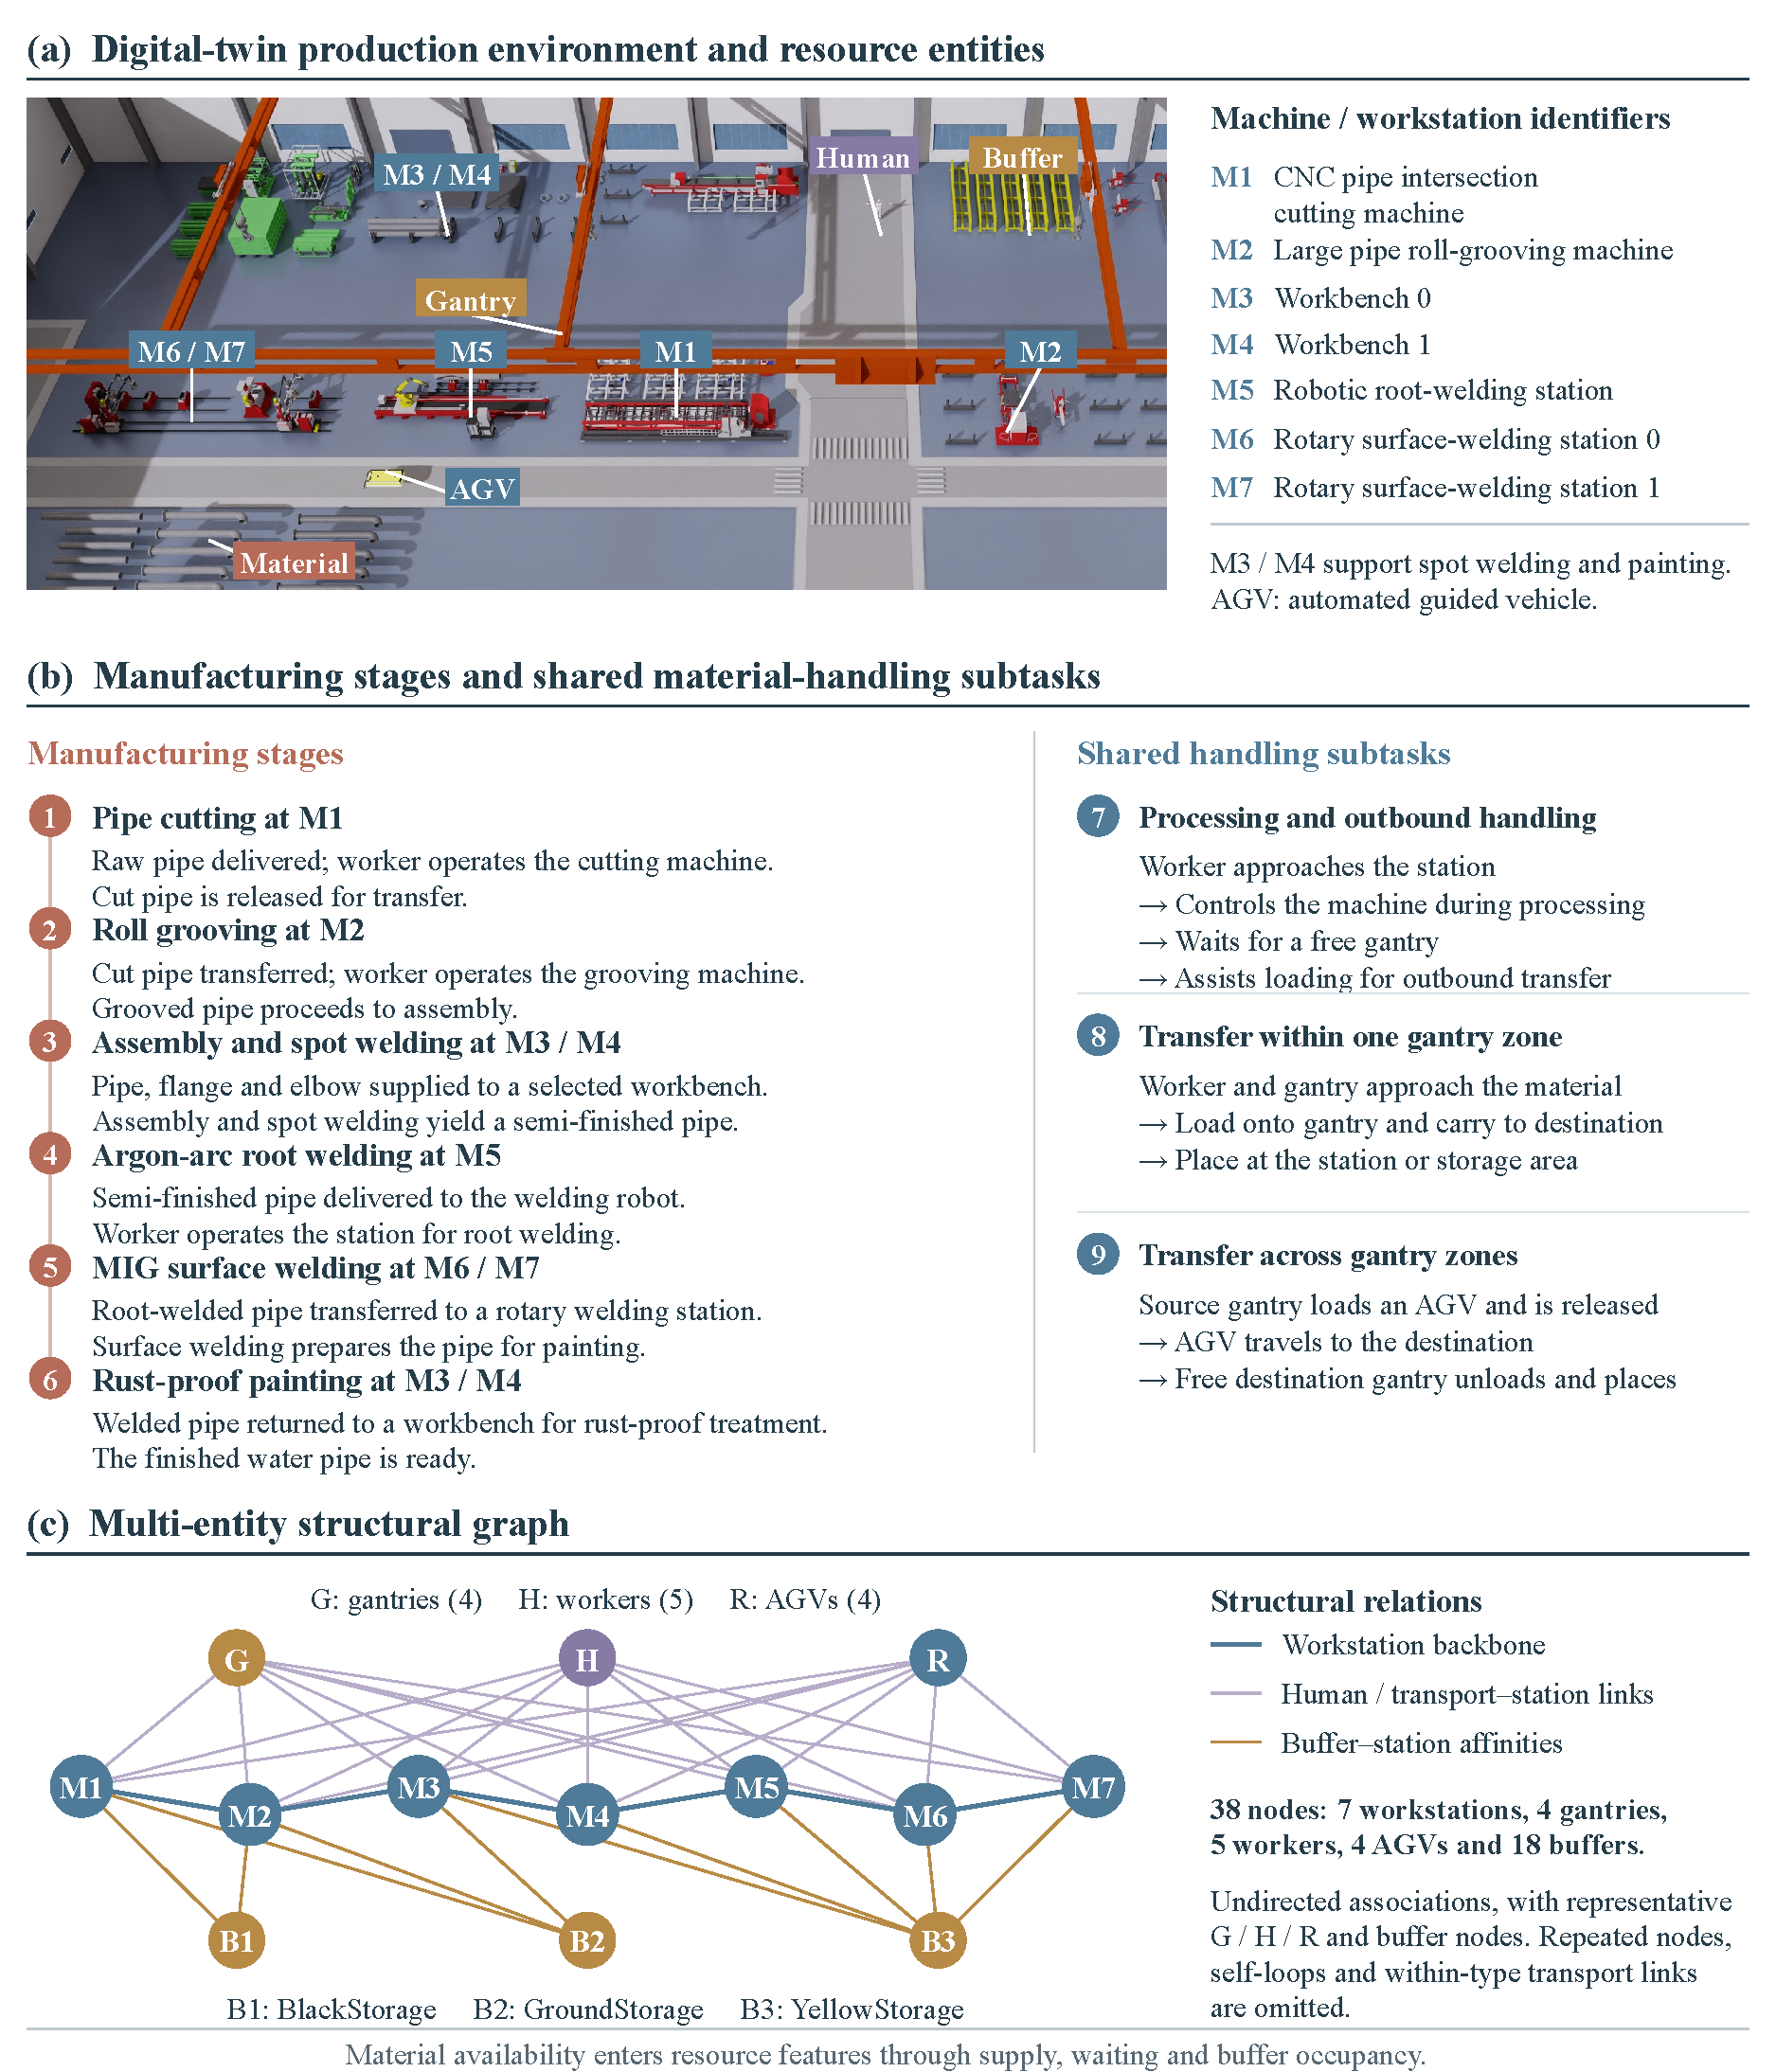
\includegraphics[width=\textwidth]{../figures/fig_experiment.pdf}
\caption{Experimental digital-twin production environment. (a)~Resource entities on the simulated line. (b)~Six manufacturing stages and shared material-handling subtasks. (c)~Multi-entity structural graph of the 38 simulated resources.}
\label{fig:experiment}
\end{figure*}

The data-generation environment exposes four disturbance dimensions and applies each dimension at three intervention levels (Table~\ref{tab:disturbance-design}). Level~0 changes episode-wide resource capacity before simulation, Level~1 perturbs sampled processing or service behaviour, and Level~2 injects temporary events during production. The platform supports intensity $I\in\{1,2,3\}$; slash-separated values in the table follow this order. The formal \texttt{dense\_i1} collection activates one dimension at a time at $I=1$, while nominal runs keep all dimensions inactive. Mixed two-, three-, and four-dimensional episodes are stored separately and are not merged into the main dataset. This separation makes the injected condition traceable without treating the disturbance dimension itself as the bottleneck or process-cause label.

\begin{table*}[t]
\centering
\caption{Four disturbance dimensions and their three intervention levels. Values separated by slashes correspond to $I=1/2/3$. One simulation step equals one logical second.}
\label{tab:disturbance-design}
\scriptsize
\setlength{\tabcolsep}{3.2pt}
\renewcommand{\arraystretch}{1.12}
\begin{tabularx}{\FullWidth}{@{}lXXX@{}}
\toprule
Dimension & L0: episode configuration & L1: sampled process variation & L2: temporary runtime events \\
\midrule
Machine / workstation & Disable workbench ws1 and rotary-welding ws1 & Processing-time noise $5/10/15$ steps; success rate $0.88/0.76/0.64$; tool wear $15/30/45$ steps per 1,000 steps & $2/(2$--$3)/(3$--$4)$ idle-station failures; additional $1$--$2/2$--$3/3$--$4$ weld or kitting quality-hold windows \\
Human & Reduce workers from 5 to $3/2/1$ & Service-time scale $1.55/2.10/2.65$; worker-specific skill range $0.8$--$1.4/0.7$--$1.6/0.6$--$1.8$; time noise $12/22/32$ steps & $2/(2$--$3)/(3$--$4)$ temporary absences, applied only when the selected worker is idle \\
Logistics & Reduce AGVs from 4 to $2/1/1$; retain all four zone gantries & Gantry-time scale $1.65/2.30/2.95$ with motion noise $10/18/26$ steps; weak background process variation & $2/(2$--$3)/(3$--$4)$ gantry or AGV freezes; at least one pulse targets an AGV while other vehicles remain active \\
Material & Keep the nominal inventory of ten pipes, flanges, and elbows; no permanent deletion & At steps 400--1,000, temporarily hide $6$--$7/7$--$8/7$--$8$ idle flanges or elbows for $1{,}400$--$2{,}200/2{,}000$--$2{,}700/2{,}500$--$3{,}200$ steps & After the opening shortage, inject $1$--$2/2$--$3/3$--$4$ complementary flange/elbow shortage pulses; pipe blanks are never hidden \\
\bottomrule
\end{tabularx}
\end{table*}

For machine, human, and logistics disturbances, every Level~2 pulse lasts at least 600 steps and the intensity-specific upper bounds are 900/1,300/1,400 steps. Event targets, start times, counts, and durations are resampled for each episode using a deterministic seed. Adjacent pulses are separated by at least 360 steps, and an event waits for an eligible idle target rather than interrupting an active operation. These controls make the injected condition long enough to survive the eight-window persistence filter while avoiding a deterministic one-to-one mapping between an injection and a labelled bottleneck.


Process-informed labels apply an eight-window persistence rule (Min8) to newly forming bottlenecks. An event already active at the last historical window is retained when at least one labelled future window remains. We evaluate three onset-cap settings, Start$\leq5$, Start$\leq10$, and Start$\leq15$, which define the admissible distance between the current window and a future event onset. The future grid and the onset cap are kept fixed within each task. A three-window start tolerance is used for strict report matching, and every window corresponds to 60~s; duration, start, and remaining-time errors are consequently reported in minutes.


\begin{table}[t]
\centering
\caption{Dataset and label protocol used in the experiments.}
\label{tab:exp-dataset}
\scriptsize
\setlength{\tabcolsep}{4pt}
\renewcommand{\arraystretch}{1.08}
\begin{tabularx}{\columnwidth}{@{}lX@{}}
\toprule
Item & Setting \\
\midrule
Dataset & \texttt{dense\_i1}, 204 episodes, 38 resources \\
Split & 140/28/36 episodes; 20,826/4,331/5,354 windows \\
Windowing & 60-s windows; 30 historical + 20 future windows \\
Targets & 15 resources: 7 machines/workbenches, 4 gantries, 4 robots \\
Event rule & Min8 persistence; Start$\leq5/10/15$ \\
Report matching & Three-window onset tolerance \\
\bottomrule
\end{tabularx}
\end{table}

\subsubsection{Baseline methods}

Four baselines cover the model families used in the common-manifest comparison. XGBoost is a gradient-boosted decision-tree predictor operating on tabular summaries, providing a non-neural reference for nonlinear feature interactions. LSTM is a recurrent predictor that models temporal dependencies in the historical sequence. BTGCN constructs a graph over production tasks and combines graph convolution with a GRU to model relational and temporal information~\cite{yin2025btgcn}. BSTAN uses graph attention with a GRU to learn adaptive neighbour contributions for blockage and starvation related prediction~\cite{lai2023bstan}. All five models use the same test-sample identities, history length, future grid, target resources, and event-label definition. Each baseline retains its corresponding input representation and training procedure.


\begin{table}[t]
\centering
\caption{Baseline families in the common-manifest comparison.}
\label{tab:exp-baselines}
\scriptsize
\setlength{\tabcolsep}{4pt}
\renewcommand{\arraystretch}{1.10}
\begin{tabularx}{\columnwidth}{@{}lXX@{}}
\toprule
Model & Core framework & Comparison role \\
\midrule
XGBoost & Gradient-boosted decision trees & Tabular predictor \\
LSTM & Long short-term memory & Recurrent temporal predictor \\
BTGCN & Graph convolution + GRU & Graph-convolutional predictor \\
BSTAN & Graph attention + GRU & Graph-attention predictor \\
\bottomrule
\end{tabularx}
\end{table}

\subsubsection{Overall experimental settings and metrics}

PHGST-DP uses five encoder blocks, an 80-dimensional latent representation, eight-dimensional Laplacian positional encoding, $4/2/2$ temporal/geographic/semantic attention heads, a four-hop geographic mask, five semantic neighbours, and 16 length-three pattern keys. AdamW is used with batch size 16, learning rate $5\times10^{-5}$, weight decay $0.05$, cosine decay to $10^{-6}$, and fourfold positive-window oversampling. Training has two stages. Stage~1 learns the bottleneck and cause heads: it is warm-started from an earlier prefix-supervised checkpoint, unfreezes the last five encoder blocks, and runs for at most 100 epochs with patience 40. The three onset caps are trained as a curriculum (Start$\leq5\rightarrow$Start$\leq10\rightarrow$Start$\leq15$). A far-onset enhancement doubles the onset loss for events starting more than 5~min ahead, sets the far-onset positive weight to $9/10/11$ for the three caps, and raises the false-alarm penalty (weights $2.5$ and $2.2$ for ordinary and hard false positives). Stage~2 freezes the encoder and every bottleneck and cause head, adds a per-workpiece rate term to the remaining-time head, and fine-tunes only that head for at most 20 epochs with validation loss as the selection criterion. This stage specializes the order-progress forecast while preserving the event and cause outputs. All runs use seed 42.


The checkpoint and report threshold are selected on the validation split. Candidate thresholds are $\{0.45,\dots,0.90,0.94\}$; selection maximizes Will15 F1 among candidates satisfying validation report precision $\geq0.80$ and recall $\geq0.70$. All three onset caps use the selected threshold of $0.94$ for testing.


Metrics follow the three prediction dimensions. Bottleneck-event evaluation combines station-level Will15 P/R/F1 with Report F1, which additionally requires an onset error within three windows. Upcoming recall uses future-event window--resource pairs whose final historical window is non-bottleneck; Ongoing recall uses pairs with an active final historical window. Start and duration MAE are measured on correctly detected events, while union duration MAE/RMSE includes missed and false events. Next-window and 20-window State F1 describe the predicted occupancy over time, including recovery. Process-cause evaluation uses accuracy and macro recall over the four supported classes. Order-completion evaluation uses remaining-time MAE at the line level.


\begin{table*}[t]
\centering
\caption{Metrics reported in the main and matched baseline experiments.}
\label{tab:exp-metrics}
\scriptsize
\setlength{\tabcolsep}{3.5pt}
\renewcommand{\arraystretch}{1.08}
\begin{tabular*}{\FullWidth}{@{\extracolsep{\fill}}lll@{}}
\toprule
Metric group & Metric & Interpretation \\
\midrule
Event & Will15 P/R/F1 & Station identification over 15 target resources \\
Event & Report F1 & Station identification with a three-window onset tolerance \\
Early warning & Upcoming / ongoing recall & Station recall: historically cold / active resources \\
State & State F1 (1-step / horizon) & Bottleneck state accuracy at one step / 20-step horizon \\
Temporal & Start MAE; duration MAE & Localization and duration error on detected events \\
Temporal & Union duration MAE/RMSE & Error including missed and false events \\
Auxiliary & Remaining-time MAE & Global order-progress estimation error \\
Auxiliary & Cause accuracy / macro recall & Four supported process-cause classes \\
\bottomrule
\end{tabular*}
\end{table*}

\subsection{Main and baseline performance comparison}

The comparison follows the three prediction dimensions delivered by PHGST-DP: the occurrence and temporal extent of a bottleneck, its associated process cause, and the remaining time to order completion. Tables~\ref{tab:comparison-event}, \ref{tab:comparison-regression}, and \ref{tab:comparison-state} compare the main model and four baselines across these outputs; Table~\ref{tab:remain-stage} reports remaining-time head specialization. The reported values are the final common-manifest results on the 5,354-window test split in Table~\ref{tab:exp-dataset}, using the same sample identities, target resources, future grid, and event-label definition for all five models.


\subsubsection{Bottleneck occurrence, onset, end, and duration}\label{sec:comparison-event}

PHGST-DP combines advance event recognition with a temporal description of the predicted constraint. Table~\ref{tab:comparison-event} reports event precision, recall, and F1; Tables~\ref{tab:comparison-regression} and \ref{tab:comparison-state} provide the corresponding onset and duration errors and future-state F1. Onset and duration characterize the timing of the predicted constraint; next-window and 20-window state predictions describe its evolution through onset, persistence, and recovery. P/R/F1 evaluate event identification, while timing errors evaluate the temporal attributes of correctly identified events.


Across the three onset caps, PHGST-DP achieves Will15 F1 of $0.805/0.783/0.772$ and Report F1 of $0.804/0.778/0.768$. The Report F1 differences from the strongest baseline are $0.102/0.167/0.191$. Upcoming recall remains $0.542/0.535/0.537$, alongside Ongoing recall of $0.937/0.939/0.930$. This combination provides advance coverage of emerging constraints while following events that are already active. The precision--recall pairs characterize the alarm operating point: PHGST-DP attains the highest recall and F1 at every cap, while the baseline precision values show their more selective reporting behaviour.


\begin{table*}[t]
\centering
\caption{Common-manifest event-identification and early-warning results. Upcoming and Ongoing R use station-level matching; bold marks the best value within each cap.}
\label{tab:comparison-event}
\scriptsize
\setlength{\tabcolsep}{3.5pt}
\renewcommand{\arraystretch}{1.08}
\begin{tabular*}{\FullWidth}{@{\extracolsep{\fill}}llrrrrrr@{}}
\toprule
Model & Start cap & P & R & Will15 F1 & Report F1 & Upcoming R & Ongoing R \\
\midrule
PHGST-DP & $\leq5$  & 79.4\% & \textbf{81.7\%} & \textbf{80.5\%} & \textbf{80.4\%} & \textbf{54.2\%} & \textbf{93.7\%} \\
XGBoost & $\leq5$  & \textbf{85.9\%} & 59.8\% & 70.5\% & 70.2\% & 6.0\% & 81.9\% \\
LSTM & $\leq5$  & 68.0\% & 51.5\% & 58.6\% & 58.3\% & 9.9\% & 68.7\% \\
BTGCN & $\leq5$  & 81.6\% & 57.0\% & 67.1\% & 66.9\% & 4.6\% & 78.6\% \\
BSTAN & $\leq5$  & 82.9\% & 59.0\% & 69.0\% & 68.7\% & 9.5\% & 79.4\% \\
\midrule
PHGST-DP & $\leq10$ & 80.6\% & \textbf{76.1\%} & \textbf{78.3\%} & \textbf{77.8\%} & \textbf{53.5\%} & \textbf{93.9\%} \\
XGBoost & $\leq10$ & 85.8\% & 48.7\% & 62.1\% & 61.1\% & 4.1\% & 80.5\% \\
LSTM & $\leq10$ & 56.1\% & 45.1\% & 50.0\% & 47.7\% & 11.2\% & 69.3\% \\
BTGCN & $\leq10$ & \textbf{88.1\%} & 44.0\% & 58.7\% & 57.9\% & 4.5\% & 72.2\% \\
BSTAN & $\leq10$ & 84.9\% & 48.8\% & 62.0\% & 60.9\% & 5.7\% & 79.6\% \\
\midrule
PHGST-DP & $\leq15$ & 80.6\% & \textbf{74.2\%} & \textbf{77.2\%} & \textbf{76.8\%} & \textbf{53.7\%} & \textbf{93.0\%} \\
XGBoost & $\leq15$ & 84.5\% & 45.3\% & 59.0\% & 57.7\% & 3.9\% & 79.6\% \\
LSTM & $\leq15$ & 62.4\% & 39.8\% & 48.6\% & 46.1\% & 10.2\% & 64.3\% \\
BTGCN & $\leq15$ & 78.8\% & 40.7\% & 53.6\% & 51.8\% & 5.4\% & 69.9\% \\
BSTAN & $\leq15$ & \textbf{85.3\%} & 40.2\% & 54.7\% & 53.4\% & 4.4\% & 70.0\% \\
\bottomrule
\end{tabular*}
\end{table*}

\begin{table*}[t]
\centering
\caption{Common-manifest temporal and continuous-value estimation results. Errors are in minutes; bold denotes the lowest value within each onset cap.}
\label{tab:comparison-regression}
\scriptsize
\setlength{\tabcolsep}{3.5pt}
\renewcommand{\arraystretch}{1.08}
\begin{tabular*}{\FullWidth}{@{\extracolsep{\fill}}llrrr@{}}
\toprule
Model & Start cap & Start MAE & Duration MAE & Remain MAE \\
\midrule
PHGST-DP & $\leq5$  & 0.127 & \textbf{1.863} & 9.600 \\
XGBoost & $\leq5$  & 0.030 & 3.264 & \textbf{5.231} \\
LSTM & $\leq5$  & 0.056 & 3.855 & 10.593 \\
BTGCN & $\leq5$  & \textbf{0.020} & 3.322 & 19.343 \\
BSTAN & $\leq5$  & 0.043 & 3.565 & 14.704 \\
\midrule
PHGST-DP & $\leq10$ & 0.227 & \textbf{1.788} & 9.270 \\
XGBoost & $\leq10$ & 0.122 & 3.210 & \textbf{5.231} \\
LSTM & $\leq10$ & 0.388 & 3.768 & 10.607 \\
BTGCN & $\leq10$ & \textbf{0.117} & 3.238 & 18.102 \\
BSTAN & $\leq10$ & 0.153 & 3.533 & 13.850 \\
\midrule
PHGST-DP & $\leq15$ & 0.227 & \textbf{1.716} & 8.910 \\
XGBoost & $\leq15$ & \textbf{0.167} & 3.170 & \textbf{5.231} \\
LSTM & $\leq15$ & 0.453 & 3.615 & 9.009 \\
BTGCN & $\leq15$ & 0.302 & 3.121 & 12.829 \\
BSTAN & $\leq15$ & 0.222 & 3.422 & 13.557 \\
\bottomrule
\end{tabular*}
\end{table*}

The temporal outputs make these alarms useful for estimating how long a resource will remain constrained. PHGST-DP's detected-event duration MAE is $1.863/1.788/1.716$~min, corresponding to reductions of $42.9\%/44.3\%/45.0\%$ relative to the lowest baseline errors. One-step State F1 reaches $0.883/0.892/0.900$, and 20-step State F1 reaches $0.525/0.589/0.610$. The latter exceeds the strongest baseline by $0.146/0.224/0.275$, extending the advantage from identifying an event to describing its future occupancy. Figure~\ref{fig:baseline-comparison} brings together report quality, advance warning, and duration estimation across the three caps.


\begin{figure*}[t]
\centering
\IfFileExists{../figures/fig_baseline_comparison.pdf}{%
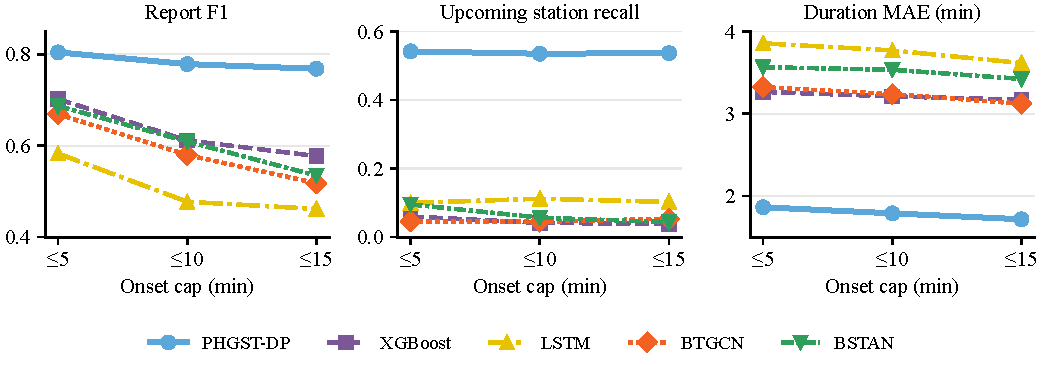
\includegraphics[width=0.96\textwidth]{../figures/fig_baseline_comparison.pdf}%
}{}
\caption{Common-manifest results across the three onset caps for Report F1, station-level Upcoming recall, and duration MAE.}
\label{fig:baseline-comparison}
\end{figure*}

Distance-resolved results further locate the model's warning capability. At Start$\leq15$, strict report recall is $0.574$, $0.522$, and $0.433$ for true onsets within 5, 6--10, and more than 10~min, respectively. Among station-matched true positives, exact-onset accuracy is $0.896/0.844/0.831$ across the three caps, and onset-bucket accuracy is $0.921/0.918/0.920$. The forecasts also cover material-handling assets: machine/gantry/robot F1 is $0.805/0.811/0.771$ at Start$\leq5$ and $0.751/0.840/0.639$ at Start$\leq15$. These results connect temporal warning to the different resources through which production constraints develop.


\subsubsection{Bottleneck process-cause prediction}\label{sec:comparison-cause}

Process-cause prediction adds an operational interpretation to the event report. PHGST-DP achieves accuracy of $0.965/0.962/0.974$ and macro recall of $0.967/0.965/0.978$ across the three caps (Table~\ref{tab:comparison-state}). These outputs associate predicted constraints with transport delay, material shortage, upstream starvation, and queue buildup, giving a process context for reviewing the affected resource and time interval. XGBoost achieves accuracy $0.990$ and macro recall $0.988$, demonstrating strong discrimination of the rule-derived cause categories; PHGST-DP integrates this explanatory output with its event and temporal forecasts.


\begin{table*}[t]
\centering
\caption{Common-manifest future-state and process-cause classification results. Bold denotes the best value within each onset cap.}
\label{tab:comparison-state}
\scriptsize
\setlength{\tabcolsep}{3.5pt}
\renewcommand{\arraystretch}{1.08}
\begin{tabular*}{\FullWidth}{@{\extracolsep{\fill}}llrrrr@{}}
\toprule
Model & Start cap & State F1 (1-step) & State F1 (20-step) & Cause acc. & Cause macro R \\
\midrule
PHGST-DP & $\leq5$  & \textbf{88.3\%} & \textbf{52.5\%} & 96.5\% & 96.7\% \\
XGBoost & $\leq5$  & 61.1\% & 37.3\% & \textbf{99.0\%} & \textbf{98.8\%} \\
LSTM & $\leq5$  & 29.5\% & 29.5\% & 93.8\% & 92.0\% \\
BTGCN & $\leq5$  & 64.3\% & 37.2\% & 90.0\% & 88.2\% \\
BSTAN & $\leq5$  & 71.9\% & 37.9\% & 95.7\% & 95.2\% \\
\midrule
PHGST-DP & $\leq10$ & \textbf{89.2\%} & \textbf{58.9\%} & 96.2\% & 96.5\% \\
XGBoost & $\leq10$ & 59.5\% & 33.7\% & \textbf{99.0\%} & \textbf{98.8\%} \\
LSTM & $\leq10$ & 27.5\% & 26.2\% & 93.6\% & 93.0\% \\
BTGCN & $\leq10$ & 56.6\% & 35.9\% & 90.7\% & 90.0\% \\
BSTAN & $\leq10$ & 63.2\% & 36.5\% & 95.9\% & 95.1\% \\
\midrule
PHGST-DP & $\leq15$ & \textbf{90.0\%} & \textbf{61.0\%} & 97.4\% & 97.8\% \\
XGBoost & $\leq15$ & 58.2\% & 32.2\% & \textbf{99.0\%} & \textbf{98.8\%} \\
LSTM & $\leq15$ & 26.8\% & 26.0\% & 94.4\% & 92.2\% \\
BTGCN & $\leq15$ & 46.1\% & 32.3\% & 90.7\% & 90.0\% \\
BSTAN & $\leq15$ & 59.3\% & 33.5\% & 95.1\% & 93.5\% \\
\bottomrule
\end{tabular*}
\end{table*}

At Start$\leq5$, PHGST-DP's cause evaluation covers 579 supported windows, with a majority-class accuracy of $0.409$. Its recalls for transport delay, material shortage, upstream starvation, and queue buildup are $0.941$, $0.976$, $0.966$, and $0.984$, respectively. The consistently high class recalls indicate that the output captures several production symptoms across the supported categories. Section~\ref{sec:supervision-analysis} examines how the cause-supervision and label-construction choices support this interpretation.


\subsubsection{Order-completion remaining-time prediction}\label{sec:comparison-remain}

Order-completion prediction extends the resource-level bottleneck report to the production line. PHGST-DP's final remaining-time MAE is $9.60/9.27/8.91$~min across the three onset caps (Table~\ref{tab:comparison-regression}). These values are the lowest among the evaluated neural models; XGBoost records $5.231$~min for its dedicated remaining-time predictor. For PHGST-DP, the order-level output supplies a completion estimate alongside the resource, timing, and cause information already available in the bottleneck report.


\begin{table}[t]
\centering
\caption{Order remaining-time MAE (min) before (stage~1) and after (stage~2) remaining-time fine-tuning. Early/middle/late windows: 2,330/1,750/1,274.}
\label{tab:remain-stage}
\scriptsize
\setlength{\tabcolsep}{3.5pt}
\renewcommand{\arraystretch}{1.08}
\begin{tabular}{llrrrr}
\toprule
Start cap & Stage & Test MAE & Early & Middle & Late \\
\midrule
$\leq5$  & 1 & 10.93 & 16.84 & 8.18 & \textbf{3.87} \\
         & 2 & \textbf{9.60} & \textbf{14.14} & \textbf{7.66} & 3.96 \\
$\leq10$ & 1 & 11.21 & 17.27 & 8.45 & 3.94 \\
         & 2 & \textbf{9.27} & \textbf{13.78} & \textbf{7.24} & \textbf{3.80} \\
$\leq15$ & 1 & 9.72 & 14.72 & 7.51 & \textbf{3.60} \\
         & 2 & \textbf{8.91} & \textbf{13.08} & \textbf{7.21} & 3.61 \\
\bottomrule
\end{tabular}
\end{table}

Head-specific fine-tuning strengthens this output while preserving the event and cause predictions. As shown in Table~\ref{tab:remain-stage}, test MAE decreases from $10.93/11.21/9.72$ to $9.60/9.27/8.91$~min, reductions of approximately $12\%/17\%/8\%$. The largest absolute gains occur in early production: MAE decreases from $16.84/17.27/14.72$ to $14.14/13.78/13.08$~min over 2,330 test windows. Late-phase MAE reaches $3.96/3.80/3.61$~min. This specialization improves completion-time estimation at the stage when substantial work remains, while the shared bottleneck forecast continues to identify local production constraints.


\subsection{Ablation study}

The ablation study links predictive performance to three design choices: heterogeneous process--logistics information, process-informed supervision, and delay-pattern conditioning. Nine configurations also examine the decoder and training choices that support advance warning (Table~\ref{tab:ablation-arms}). Dataset, target resources, label rules, and validation-based threshold selection follow the main experiment; the selected threshold is $0.94$ except for NoFarBoost ($0.90/0.88/0.94$). Initialization and training budgets are listed for each arm: the structural variants use up to 50 epochs, while PHGST-DP uses warm-start curriculum training with a 100-epoch budget. These comparisons assess the resulting model configurations; the matched-budget Cause$\times$State experiment separately isolates auxiliary-supervision effects. Remaining-time comparisons use the stage-1 reference, before head-specific fine-tuning.


\begin{table*}[t]
\centering
\caption{Ablation arms. ``Scratch'' arms are trained from random initialization for at most 50 epochs; ``curriculum'' arms initialize the Start$\leq10/15$ runs from the preceding cap.}
\label{tab:ablation-arms}
\scriptsize
\setlength{\tabcolsep}{3.5pt}
\renewcommand{\arraystretch}{1.08}
\begin{tabular*}{\FullWidth}{@{\extracolsep{\fill}}llll@{}}
\toprule
Arm & Contribution & Change relative to the retained model & Training \\
\midrule
NoGraph & Heterogeneous graph & Self-loop adjacency only; no factory edges & Scratch, 50 ep. \\
NoGroup & Heterogeneous graph & One linear projection of the 27 channels instead of six semantic groups & Scratch, 50 ep. \\
NoCross & Heterogeneous graph & Within-type edges only; cross-type semantic attention masked & Scratch, 50 ep. \\
NoInfo & Heterogeneous graph & Only machines observed; non-machine features and five coupling channels zeroed & Scratch, 50 ep. \\
MachineOnly & Heterogeneous graph & NoCross and NoInfo combined & Scratch, 50 ep. \\
NoCluster & Cause/regime components & No cause supervision, no regime-cluster fusion, contrast, or recall lift & Scratch, 50 ep. \\
NoPattern & Delay propagation & Delay-aware pattern matching disabled & Scratch $\rightarrow$ curriculum, 50 ep. \\
NoSplit & Decoder & One shared will head for continuing and new events & Scratch $\rightarrow$ curriculum, 50 ep. \\
NoFarBoost & Training & Far-onset weighting removed; earlier false-alarm penalty and report-F1 selection & Warm start, 100 ep. \\
\bottomrule
\end{tabular*}
\end{table*}

\begin{figure*}[t]
\centering
\IfFileExists{../figures/fig_ablation_delta.pdf}{%
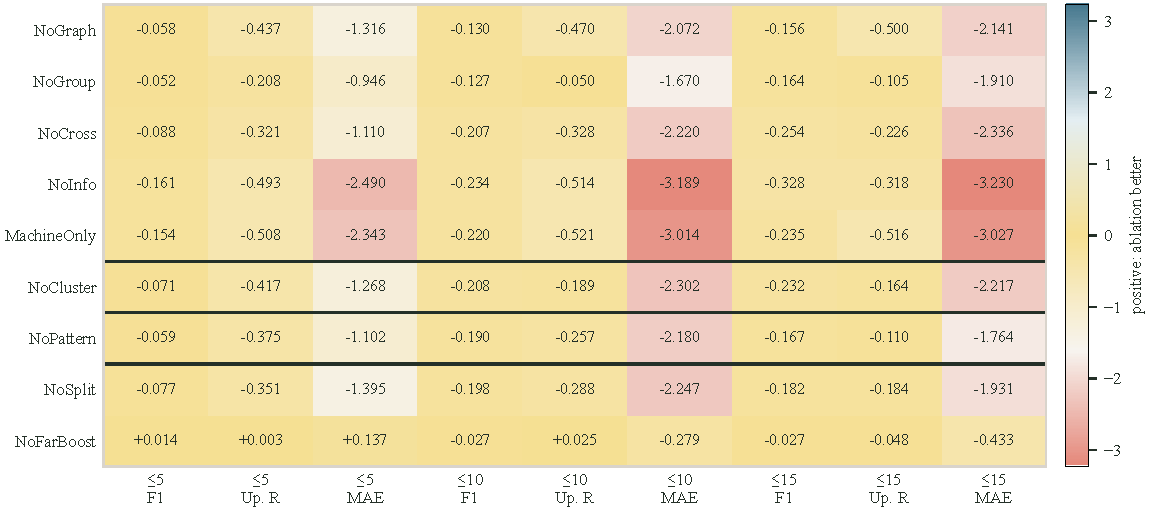
\includegraphics[width=0.96\textwidth]{../figures/fig_ablation_delta.pdf}%
}{}
\caption{Configuration-level change relative to PHGST-DP on the shared 5,354-window test split. Rows are grouped, from top to bottom, into heterogeneous-graph, supervision, delay-pattern, and decoder arms. For Report F1 and Upcoming recall the cell is ablation minus Full; for union duration MAE (min) it is Full minus ablation, so a positive value means the ablation scores better. Steel is positive and coral is negative. Training budgets and, for NoInfo and MachineOnly, event pools differ, so the matrix is not a single-factor causal estimate.}
\label{fig:ablation-overview}
\end{figure*}

PHGST-DP preserves event accuracy as the onset range expands (Figure~\ref{fig:ablation-overview}). The heatmap gives the signed gap from Full: most removed components lower Report F1 and Upcoming recall and raise union duration error, while NoFarBoost is slightly better at Start$\leq5$ under its own threshold. From Start$\leq5$ to Start$\leq15$, Full Will15 F1 changes from $0.805$ to $0.772$, and union duration MAE from $4.17$ to $4.43$~min. The structural and entity variants exhibit larger changes, with F1 reductions of $0.08$--$0.16$ and MAE increases of $0.8$--$1.5$~min under their listed training configurations. The following analyses identify which aspects of warning, state tracking, and interpretation distinguish the full model.


\begin{figure*}[t]
\centering
\IfFileExists{../figures/fig_remain_dumbbell.pdf}{%
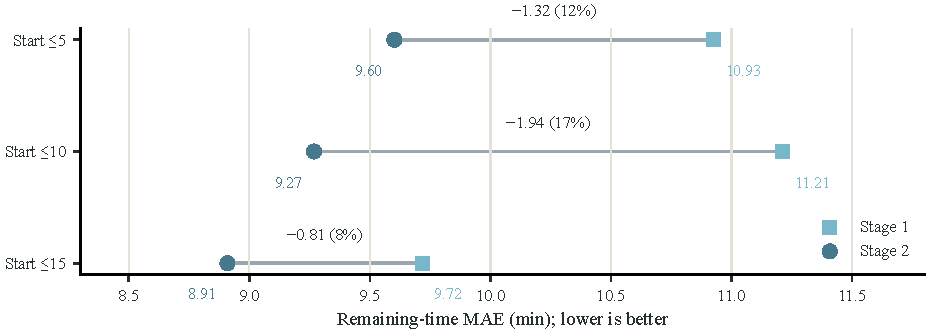
\includegraphics[width=0.82\textwidth]{../figures/fig_remain_dumbbell.pdf}%
}{}
\caption{Order remaining-time MAE of Full PHGST-DP before and after remaining-time fine-tuning. The square is stage 1 and the circle is stage 2; the label is the absolute and relative drop. Other arms are not shown, because they do not share this two-stage budget.}
\label{fig:remain-bars}
\end{figure*}


\subsubsection{Heterogeneous graph and multi-entity information}

This experiment examines the value of observing heterogeneous resources and exchanging information across their process relations (Table~\ref{tab:entity-ablation-new}). NoGraph and NoGroup remove the factory graph and grouped embedding, respectively. NoCross retains all observations and restricts interaction to the same resource type. NoInfo uses machine observations with five coupling channels masked: route delay, inbound waiting, shortage propagation, blocked-minus-starved time, and labour saturation. MachineOnly combines the NoCross and NoInfo restrictions.


\begin{table*}[t]
\centering
\caption{Ablation of the heterogeneous graph, grouped embedding, and multi-entity information. Dur.\ MAE is the union duration MAE (min), which penalizes misses and false alarms. NoInfo and MachineOnly observe a smaller event pool (955/1,225/1,331 instead of 1,102/1,372/1,478 true events).}
\label{tab:entity-ablation-new}
\scriptsize
\setlength{\tabcolsep}{3.5pt}
\renewcommand{\arraystretch}{1.05}
\begin{tabular*}{\FullWidth}{@{\extracolsep{\fill}}llrrrrrr@{}}
\toprule
Arm & Start cap & P & Will15 F1 & Upcoming R & Ongoing R & State F1 (1-step) & Dur.\ MAE \\
\midrule
Full & $\leq5$ & 79.4\% & \textbf{80.5\%} & \textbf{54.2\%} & 93.7\% & \textbf{88.3\%} & \textbf{4.17} \\
NoGraph &  & 83.2\% & 74.7\% & 10.4\% & 93.0\% & 87.3\% & 5.48 \\
NoGroup &  & 76.6\% & 76.1\% & 33.3\% & \textbf{94.1\%} & 83.5\% & 5.11 \\
NoCross &  & 75.0\% & 72.3\% & 22.0\% & 90.7\% & 81.2\% & 5.28 \\
NoInfo &  & 77.0\% & 64.4\% & 4.9\% & 89.9\% & 69.9\% & 6.66 \\
MachineOnly &  & 79.8\% & 65.0\% & 3.3\% & 90.3\% & 70.9\% & 6.51 \\
\midrule
Full & $\leq10$ & 80.6\% & \textbf{78.3\%} & \textbf{53.5\%} & 93.9\% & \textbf{89.2\%} & \textbf{4.38} \\
NoGraph &  & 82.1\% & 65.1\% & 6.5\% & 91.1\% & 84.4\% & 6.46 \\
NoGroup &  & 60.5\% & 66.8\% & 48.5\% & \textbf{94.9\%} & 82.6\% & 6.05 \\
NoCross &  & 59.6\% & 59.5\% & 20.7\% & 89.6\% & 75.9\% & 6.60 \\
NoInfo &  & 75.9\% & 54.5\% & 2.1\% & 89.6\% & 68.4\% & 7.57 \\
MachineOnly &  & 82.0\% & 55.9\% & 1.4\% & 90.1\% & 70.8\% & 7.40 \\
\midrule
Full & $\leq15$ & 80.6\% & \textbf{77.2\%} & \textbf{53.7\%} & \textbf{93.0\%} & \textbf{90.0\%} & \textbf{4.43} \\
NoGraph &  & 85.1\% & 61.6\% & 3.7\% & 89.2\% & 86.5\% & 6.57 \\
NoGroup &  & 56.7\% & 62.3\% & 43.2\% & 92.7\% & 81.9\% & 6.34 \\
NoCross &  & 51.8\% & 56.3\% & 31.1\% & 89.7\% & 76.0\% & 6.77 \\
NoInfo &  & 46.6\% & 49.0\% & 21.8\% & 92.2\% & 59.6\% & 7.66 \\
MachineOnly &  & 80.2\% & 53.4\% & 2.1\% & 91.2\% & 70.6\% & 7.46 \\
\bottomrule
\end{tabular*}
\end{table*}

Cross-resource information is most closely associated with advance warning. PHGST-DP's Upcoming recall is $0.542/0.535/0.537$, compared with $0.049/0.021/0.218$ for NoInfo and $0.033/0.014/0.021$ for MachineOnly. Ongoing recall stays near or above $0.89$ across these configurations, locating the principal difference in the recognition of emerging constraints. The full model also covers non-machine targets: at Start$\leq5$, gantry F1 is $0.811$, compared with $0.082$ for NoInfo and $0$ for MachineOnly. NoGraph records Upcoming recall of $0.104/0.065/0.037$, and NoCross lies between the observation-restricted configurations and PHGST-DP. NoGroup records Upcoming recall of $0.333/0.485/0.432$ with precision $0.605/0.567$ at the longer caps, consistent with grouped embedding helping distinguish precursors from false alarms. The device traces in Figure~\ref{fig:key-device-entity} connect these differences to event persistence: PHGST-DP identifies both intervals about 5~min before NoInfo and MachineOnly, whose duration estimates remain at 6--8~min during the 20-min target segment; NoCross reaches 14~min before decaying to about 8~min.


\begin{figure*}[t]
\centering
\IfFileExists{../figures/key_device_entity.pdf}{%
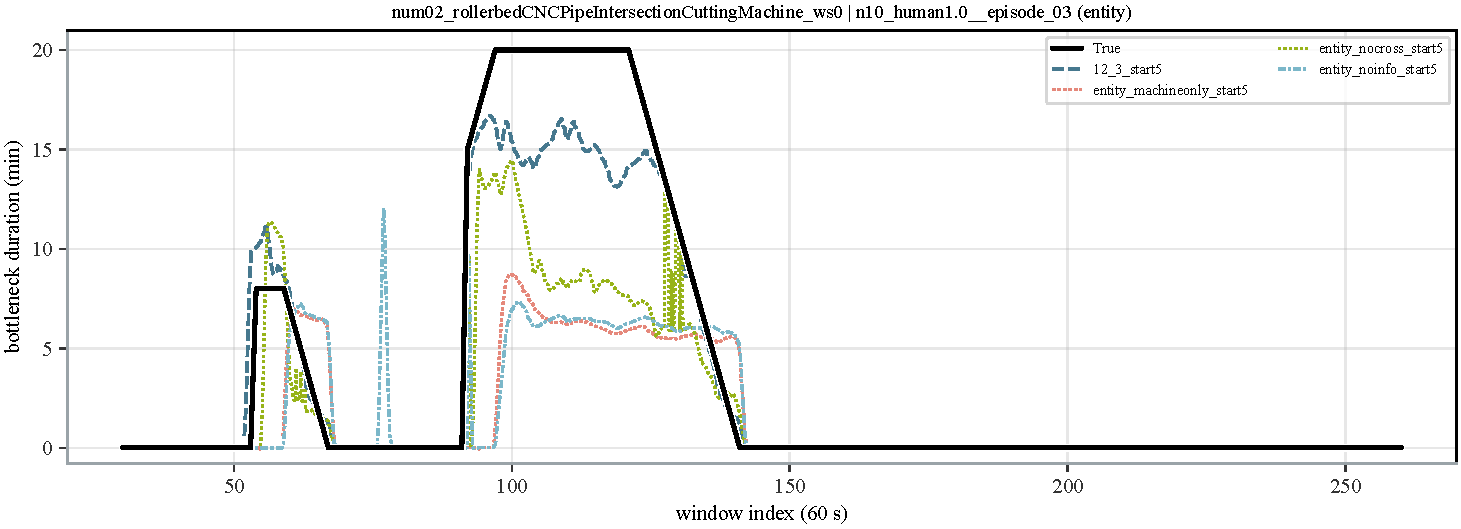
\includegraphics[width=0.96\textwidth]{../figures/key_device_entity.pdf}%
}{}
\caption{Key-device duration traces (Start$\leq5$) for the retained model and the multi-entity ablations on \texttt{num02\_rollerbedCNCPipeIntersectionCuttingMachine\_ws0}, episode \texttt{n10\_human1.0\_\_episode\_03}.}
\label{fig:key-device-entity}
\end{figure*}

\subsubsection{Process-informed supervision analysis}\label{sec:supervision-analysis}

Process-informed supervision connects the event representation to production meaning. The analysis focuses on event and state reporting under the complete supervision configuration, cause accuracy under a matched training budget, and alignment between process-informed label rankings and intervention-sensitive resources. These experiments answer different questions and are therefore interpreted separately.


\paragraph*{(1) Effects of supervision components.}
The full configuration combines event recognition with process-cause and regime information. The NoCluster comparison retains Ops event labels and jointly removes cause supervision, history-regime fusion into the event head, cluster contrastive loss, and abnormal-cluster recall lift (Table~\ref{tab:group-ablation}). Across the three onset caps, PHGST-DP records higher event F1, upcoming-event recall, and next-window state F1, together with lower union and detected-event duration errors. This is a configuration-level comparison under the schedules in Table~\ref{tab:ablation-arms}, rather than a single-factor causal estimate; the matched-budget experiment below isolates the explanatory benefit of cause supervision.


\begin{table*}[t]
\centering
\caption{Event, state, and duration metrics for the complete process-informed supervision configuration and NoCluster. Dur.\ MAE is the union error (min); Dur.\ MAE (tp) is computed on correctly reported events only.}
\label{tab:group-ablation}
\scriptsize
\setlength{\tabcolsep}{3.5pt}
\renewcommand{\arraystretch}{1.08}
\begin{tabular*}{\FullWidth}{@{\extracolsep{\fill}}llrrrrr@{}}
\toprule
Arm & Start cap & Will15 F1 & Upcoming R & State F1 (1-step) & Dur.\ MAE & Dur.\ MAE (tp) \\
\midrule
Full & $\leq5$ & \textbf{80.5\%} & \textbf{54.2\%} & \textbf{88.3\%} & \textbf{4.17} & \textbf{1.86} \\
NoCluster & & 73.5\% & 12.5\% & 84.1\% & 5.43 & 2.89 \\
\midrule
Full & $\leq10$ & \textbf{78.3\%} & \textbf{53.5\%} & \textbf{89.2\%} & \textbf{4.38} & \textbf{1.79} \\
NoCluster & & 60.2\% & 34.6\% & 78.9\% & 6.69 & 2.40 \\
\midrule
Full & $\leq15$ & \textbf{77.2\%} & \textbf{53.7\%} & \textbf{90.0\%} & \textbf{4.43} & \textbf{1.72} \\
NoCluster & & 57.7\% & 37.3\% & 81.9\% & 6.65 & 2.30 \\
\bottomrule
\end{tabular*}
\end{table*}

Cause supervision provides a direct gain in process interpretation under matched training conditions (Table~\ref{tab:matched-cause-state}). With Ops labels, a common data split, Start$\leq5$, seed 42, random initialization, and a 50-epoch budget, the cause-enabled configurations attain the highest cause accuracy. The corresponding training logs show that station identification remains at a similar level, so the measured benefit is localized to the explanatory output. Cause accuracy is retained as the direct measure of this explanatory benefit; State denotes the historical regime-state embedding and its representation objective.


\begin{table}[t]
\centering
\caption{Cause accuracy in the matched-budget auxiliary-component study at Start$\leq5$ (seed 42; 50 epochs). State denotes regime-state embedding.}
\label{tab:matched-cause-state}
\scriptsize
\setlength{\tabcolsep}{3.5pt}
\renewcommand{\arraystretch}{1.08}
\begin{tabular*}{\columnwidth}{@{\extracolsep{\fill}}lr@{}}
\toprule
Configuration & Cause accuracy \\
\midrule
Backbone & 19.5\% \\
+Cause & \textbf{89.5\%} \\
+State & 18.5\% \\
+Cause+State & \textbf{89.5\%} \\
\bottomrule
\end{tabular*}
\end{table}

% Evidence: isaac_factory origin/dev_tyx, 8767583f3ed6392cfd8061d4a80de94fcfb9d7a0.
% Source: bottleneck ground-truth validity notes (2026-10-14), checked against label/evaluation code.
% Imported summary values: experiments/data/label_validity_dev_tyx_8767583.json.
\paragraph*{(2) Validation against production sensitivity.}
Production sensitivity provides an operational criterion for bottleneck labels: prioritizing resources whose temporary acceleration shortens order completion. Counterfactual replay compares a service intervention with the unchanged production trajectory from the same saved state. This connects the label ranking to the consequence of a resource-level action.


At a saved simulation state $t$, each of seven machine/workstation candidates receives a separate service-bundle intervention. Machine processing and its associated human service use a duration scale of $0.8$, equivalent to a $1.25\times$ service rate, for 1,200 simulation steps. Baseline and intervention branches start from the same saved state and random-number state and run to order completion. The counterfactual sensitivity is
\begin{equation}
S_i(t)=M_{\mathrm{base}}(t)-M_{i,0.8}(t),
\end{equation}
where $M$ denotes order-completion time. Positive $S_i(t)$ indicates that temporarily accelerating resource $i$ shortens the order. Each label method ranks candidates using its maximum evidence over the last three fully observed windows before $t$.


Ops yields the highest point estimates on all five sensitivity-alignment metrics in the three-episode disturbance-free pilot (Table~\ref{tab:label-oracle-pilot}). NDCG@3 measures ranking quality using positive sensitivity as relevance; Positive Recall@$k$ measures coverage of the oracle's $k$ highest positive-sensitivity resources by the first $k$ candidates. Weighted Recall@3 gives the fraction of total positive sensitivity captured by the first three candidates, and Coverage@3$_{0.9}$ covers resources satisfying $S_i\geq0.9\max_j S_j$. Ops reaches NDCG@3 $0.531$ and Weighted Recall@3 $0.716$, compared with $0.495$ and $0.585$ for Queue-Wait. The mean weighted coverage of positive sensitivity by its top-three candidates is $71.6\%$ under this pilot protocol. Early-, middle-, and late-stage NDCG@3 values are $0.421/0.339/0.770$, with the strongest alignment near order completion.


\begin{table*}[t]
\centering
\caption{Counterfactual sensitivity alignment in the exploratory pilot (three disturbance-free episodes). Higher is better; bold marks the highest point estimate.}
\label{tab:label-oracle-pilot}
\scriptsize
\setlength{\tabcolsep}{3.5pt}
\renewcommand{\arraystretch}{1.08}
\begin{tabular*}{\FullWidth}{@{\extracolsep{\fill}}lrrrrr@{}}
\toprule
Label method & NDCG@3 & Positive R@2 & Positive R@3 & Weighted R@3 & Coverage@3$_{0.9}$ \\
\midrule
Ops & \textbf{.531} & \textbf{.556} & \textbf{.685} & \textbf{.716} & \textbf{.722} \\
TPM & .372 & .278 & .389 & .421 & .444 \\
Active Period & .382 & .278 & .315 & .377 & .389 \\
Utilization & .183 & .222 & .204 & .230 & .222 \\
Queue-Wait & .495 & .444 & .556 & .585 & .611 \\
\bottomrule
\end{tabular*}
\end{table*}

The same development export separates representation separability from cause identification (Figure~\ref{fig:label-validity} and Table~\ref{tab:label-boundary}). On a shared raw-last representation, Active Period records the highest macro-F1 ($0.628$), balanced accuracy ($0.904$) and AUROC ($0.963$); Ops is highest only on station macro-F1 ($0.619$). Queue-Wait records the highest cause macro-F1 ($0.940$), against $0.885$ for Active Period, on 3,245 test windows. These comparisons use one seed and are not ablations of the retained checkpoint, which is trained with the Ops persistence rule. A label that aligns with the pilot's intervention ranking therefore need not be the most separable state, and the most separable state need not be the best cause target.

\begin{figure*}[t]
\centering
\IfFileExists{../figures/fig_label_validity.pdf}{%
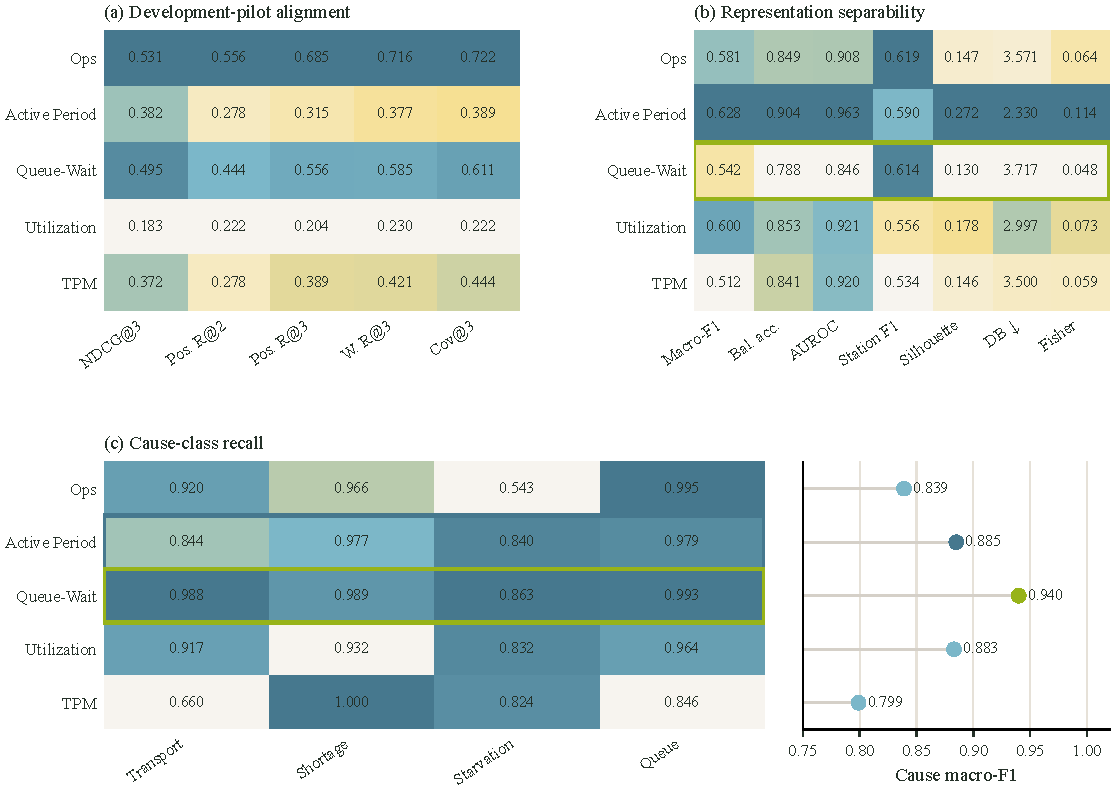
\includegraphics[width=0.96\textwidth]{../figures/fig_label_validity.pdf}%
}{}
\caption{Label-method comparison from the fixed development export (seed 42). (a) Counterfactual alignment on three disturbance-free episodes; higher is better. (b) Representation separability; colour is scaled within each column, and Davies--Bouldin is marked as lower-better. (c) Cause-class recall, with cause macro-F1 at right. Active Period is outlined in steel blue and Queue-Wait in olive. This is not an ablation of PHGST-DP.}
\label{fig:label-validity}
\end{figure*}

\begin{table*}[t]
\centering
\caption{Recorded advantages and limits of the five label methods in the development export. Bold marks the highest point estimate in a column. The retained PHGST-DP runs use the Ops persistence rule; this table does not reselect that rule.}
\label{tab:label-boundary}
\scriptsize
\setlength{\tabcolsep}{3.5pt}
\renewcommand{\arraystretch}{1.08}
\begin{tabular*}{\FullWidth}{@{\extracolsep{\fill}}lrrrrrp{0.28\FullWidth}@{}}
\toprule
Label method & Macro-F1 & Bal.\ acc. & AUROC & Station F1 & Cause macro-F1 & Main limit in this export \\
\midrule
Ops & .581 & .849 & .908 & \textbf{.619} & .839 & Lowest positive rate (.015); separability below Active Period \\
Active Period & \textbf{.628} & \textbf{.904} & \textbf{.963} & .590 & .885 & Weaker pilot alignment (NDCG@3 .382) \\
Queue-Wait & .542 & .788 & .846 & .614 & \textbf{.940} & Highest positive rate (.087) \\
Utilization & .600 & .853 & .921 & .556 & .883 & Weakest pilot alignment (NDCG@3 .183) \\
TPM & .512 & .841 & .920 & .534 & .799 & Lowest separability macro-F1 \\
\bottomrule
\end{tabular*}
\end{table*}

These exploratory estimates support production sensitivity as a distinct dimension of supervision quality. All five retained soft-alignment metrics favour Ops in this pilot, but the metric set was finalized after inspecting the pilot and Holm-adjusted paired comparisons do not reject the null hypotheses. The independent full-Oracle evaluation has not been run; the numerical ordering is therefore interpreted only as a development result for disturbance-free episodes, not as proof of general superiority across operating conditions.


\subsubsection{Delay-pattern conditioning}

Delay-pattern conditioning supports warnings that precede the visible bottleneck state. PHGST-DP records Upcoming recall of $0.542/0.535/0.537$, compared with $0.167/0.278/0.427$ for NoPattern, which retains the graph and attention branches while disabling the matching of recent patches to clustered pattern keys (Table~\ref{tab:delay-ablation-new}). For events starting more than 10~min ahead, strict report recall is $0.433$ versus $0.163$. This distance-resolved result is consistent with the role of historical patterns in representing delayed propagation. Queue-buildup cause recall is $0.984$ for PHGST-DP at Start$\leq5$, compared with $0.145$ for NoPattern; NoPattern records $0.476/0.573$ at the longer caps. The stage-1 remaining-time reference also records MAE $10.93/11.21/9.72$~min, compared with $18.62/13.35/11.06$~min for NoPattern, linking temporal context to order-progress estimation.


\begin{table*}[t]
\centering
\caption{Ablation of delay-pattern conditioning. $R_{\mathrm{up,rep}}$ is strict report recall within the stated onset-distance bin. Remain MAE (min) is compared with the stage-1 model, which, like the ablation, has no remaining-time fine-tuning.}
\label{tab:delay-ablation-new}
\scriptsize
\setlength{\tabcolsep}{3.5pt}
\renewcommand{\arraystretch}{1.08}
\begin{tabular*}{\FullWidth}{@{\extracolsep{\fill}}llrrrrrrr@{}}
\toprule
Arm & Start cap & Will15 F1 & Report F1 & Upcoming R & $R_{\mathrm{up,rep}}^{6\text{--}10}$ & $R_{\mathrm{up,rep}}^{>10}$ & Queue R & Remain MAE \\
\midrule
Full (stage 1) & $\leq5$ & \textbf{80.5\%} & \textbf{80.4\%} & \textbf{54.2\%} & --- & --- & \textbf{98.4\%} & \textbf{10.93} \\
NoPattern & & 74.8\% & 74.5\% & 16.7\% & --- & --- & 14.5\% & 18.62 \\
\midrule
Full (stage 1) & $\leq10$ & \textbf{78.3\%} & \textbf{77.8\%} & \textbf{53.5\%} & \textbf{46.6\%} & --- & \textbf{98.4\%} & \textbf{11.21} \\
NoPattern & & 60.7\% & 58.8\% & 27.8\% & 14.9\% & --- & 47.6\% & 13.35 \\
\midrule
Full (stage 1) & $\leq15$ & \textbf{77.2\%} & \textbf{76.8\%} & \textbf{53.7\%} & \textbf{52.2\%} & \textbf{43.3\%} & \textbf{98.4\%} & \textbf{9.72} \\
NoPattern & & 61.6\% & 60.1\% & 42.7\% & 39.6\% & 16.3\% & 57.3\% & 11.06 \\
\bottomrule
\end{tabular*}
\end{table*}

\subsubsection{Decoder and training components}

The decoder and training comparisons examine two requirements of advance warning: distinguishing new events from continuing events and maintaining sensitivity to distant onsets. NoSplit replaces the continuation and onset heads with one shared head. NoFarBoost uses the configuration without far-onset weighting, together with the earlier false-alarm penalty and report-F1 checkpoint criterion. Table~\ref{tab:decoder-ablation} reports the resulting operating points.


\begin{table*}[t]
\centering
\caption{Ablation of the split event heads and the far-onset enhancement. Distance-specific $R_{\mathrm{up,rep}}$ additionally requires the three-window onset tolerance. Thr is the validation-selected report threshold.}
\label{tab:decoder-ablation}
\scriptsize
\setlength{\tabcolsep}{3.5pt}
\renewcommand{\arraystretch}{1.08}
\begin{tabular*}{\FullWidth}{@{\extracolsep{\fill}}llrrrrrrr@{}}
\toprule
Arm & Start cap & Thr & P & Will15 F1 & Upcoming R & $R_{\mathrm{up,rep}}^{>10}$ & Ongoing R & Dur.\ MAE \\
\midrule
Full & $\leq5$ & 94.0\% & 79.4\% & 80.5\% & 54.2\% & --- & \textbf{93.7\%} & 4.17 \\
NoFarBoost & & 90.0\% & \textbf{83.2\%} & \textbf{82.0\%} & \textbf{54.5\%} & --- & 92.3\% & \textbf{4.03} \\
NoSplit & & 94.0\% & 75.2\% & 72.9\% & 19.0\% & --- & 93.5\% & 5.56 \\
\midrule
Full & $\leq10$ & 94.0\% & \textbf{80.6\%} & \textbf{78.3\%} & 53.5\% & --- & 93.9\% & \textbf{4.38} \\
NoFarBoost & & 88.0\% & 75.0\% & 75.7\% & \textbf{56.0\%} & --- & 92.3\% & 4.66 \\
NoSplit & & 94.0\% & 56.4\% & 59.9\% & 24.7\% & --- & \textbf{94.7\%} & 6.63 \\
\midrule
Full & $\leq15$ & 94.0\% & \textbf{80.6\%} & \textbf{77.2\%} & \textbf{53.7\%} & \textbf{43.3\%} & 93.0\% & \textbf{4.43} \\
NoFarBoost & & 94.0\% & 77.2\% & 74.3\% & 48.9\% & 24.0\% & 92.5\% & 4.87 \\
NoSplit & & 94.0\% & 55.9\% & 60.7\% & 35.3\% & 12.5\% & \textbf{95.1\%} & 6.36 \\
\bottomrule
\end{tabular*}
\end{table*}

Separating onset and continuation decisions gives PHGST-DP Upcoming recall of $0.542/0.535/0.537$, compared with $0.190/0.247/0.353$ for the shared head; NoSplit's Ongoing recall remains $0.935$--$0.951$. The contrast localizes the value of separate decisions to emerging events. Far-onset enhancement concentrates its benefit at the 10- and 15-min caps, where PHGST-DP records Will15 F1 $0.783/0.772$ and union duration MAE $4.38/4.43$~min, compared with $0.757/0.743$ and $4.66/4.87$~min for NoFarBoost. Strict report recall for events beyond 10~min rises from $0.240$ to $0.433$. At the 5-min cap, NoFarBoost records F1 $0.820$ and union MAE $4.03$~min, at threshold $0.90$ versus $0.94$ for PHGST-DP. This range-dependent pattern motivates the enhancement for longer warning distances. On the key-device trace (Figures~\ref{fig:key-device-struct-graph} and \ref{fig:key-device-struct-mech}), PHGST-DP reaches 15--17~min during the 20-min target segment and follows its decay; the structural variants peak at 12--14.5~min and show post-event spikes.


\begin{figure*}[t]
\centering
\IfFileExists{../figures/key_device_struct_graph.pdf}{%
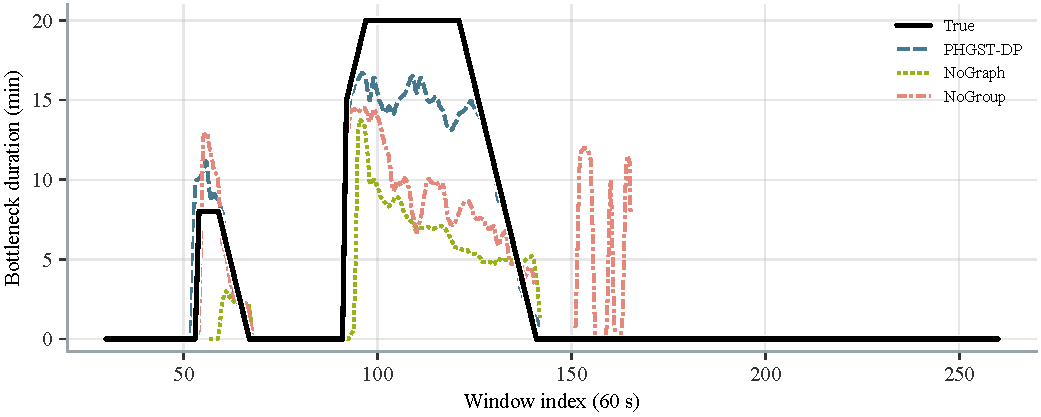
\includegraphics[width=0.96\textwidth]{../figures/key_device_struct_graph.pdf}%
}{}
\caption{Key-device duration traces (Start$\leq5$) for the retained model and the heterogeneous-graph ablations (NoGraph, NoGroup) on the same device and episode as Figure~\ref{fig:key-device-entity}.}
\label{fig:key-device-struct-graph}
\end{figure*}

\begin{figure*}[t]
\centering
\IfFileExists{../figures/key_device_struct_mech.pdf}{%
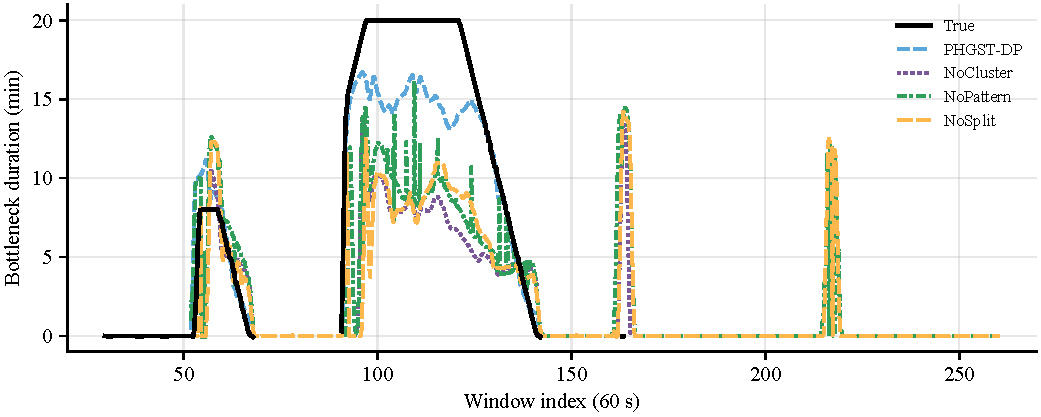
\includegraphics[width=0.96\textwidth]{../figures/key_device_struct_mech.pdf}%
}{}
\caption{Key-device duration traces (Start$\leq5$) for the retained model and the cause, delay-pattern, and decoder ablations (NoCluster, NoPattern, NoSplit) on the same device and episode as Figure~\ref{fig:key-device-entity}.}
\label{fig:key-device-struct-mech}
\end{figure*}

\subsection{Case study and process traceability}

The case study shows how an event report follows bottleneck onset, persistence, and recovery on a production resource. The selected roller-bed CNC pipe-intersection cutting machine (\texttt{num02}) contributes 301 event-positive window--resource pairs in the test set. Device and episode selection follows a fixed rule: among devices with at least the median event count, select the device with the most events in one episode (ties resolved by PHGST-DP one-step F1), then select its episode with the most and longest bottleneck segments. The resulting episode, \texttt{n10\_human1.0\_\_episode\_03}, contains an approximately 8-min bottleneck and a 49-min bottleneck, with the duration target capped at the 20-min prediction horizon. PHGST-DP detects both intervals and tracks their recovery (Figure~\ref{fig:key-device-main}). The short event is reported about 1~min in advance with a 10--11~min duration estimate; the long event's onset is aligned, and its declining duration is followed. The capped portion is predicted at 13--17~min, and state mismatches occur at onset and recovery boundaries (1--2 windows each). The trace illustrates how the report combines event notification with a continuously updated duration estimate.

\begin{figure*}[t]
\centering
\IfFileExists{../figures/fig_key_device_timeline.pdf}{%
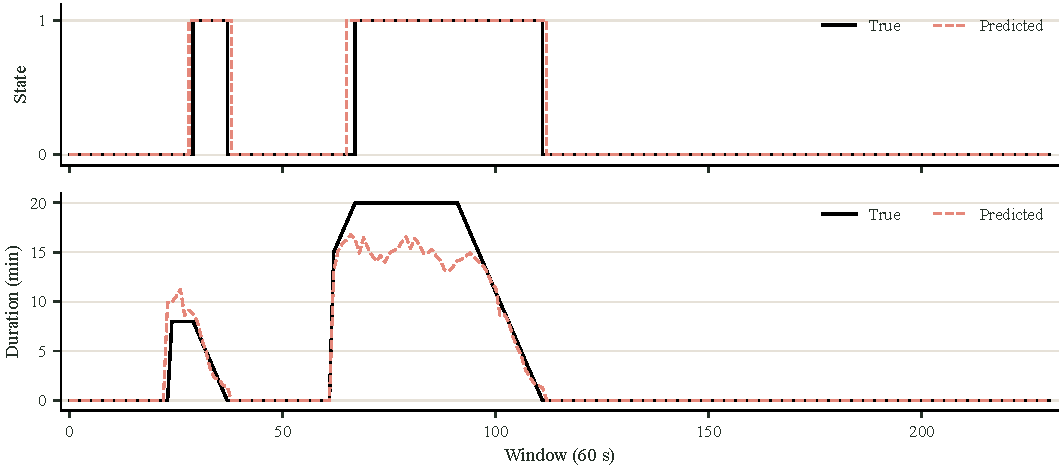
\includegraphics[width=0.96\textwidth]{../figures/fig_key_device_timeline.pdf}%
}{}
\caption{PHGST-DP state and duration on \texttt{num02}, episode \texttt{n10\_human1.0\_\_episode\_03}, Start$\leq5$. Black solid lines are the targets; coral dashed lines are the predictions. The local export does not include disturbance intervals or cause marks, so those bands are not drawn.}
\label{fig:key-device-main}
\end{figure*}

Figure~\ref{fig:key-device-baselines} places PHGST-DP at the upper left and the four baselines below, with an independent state--duration pair for each model on the same device and episode. The upper-right pair enlarges windows 20--115, shaded in the full trajectory, to show the short and long bottleneck intervals and their recovery boundaries. Both views retain the same vertical scales and window indices. Black solid lines show the targets and dashed lines show predictions; all panels count windows from the same first forecast window after the 30-window history. PHGST-DP maintains continuous state coverage over both bottleneck intervals and follows the duration decline towards recovery. The baseline panels make differences in state continuity and duration tracking visible on the same trajectory. The aggregate event and temporal results are reported in Tables~\ref{tab:comparison-event} and \ref{tab:comparison-regression}.


\begin{figure*}[p]
\centering
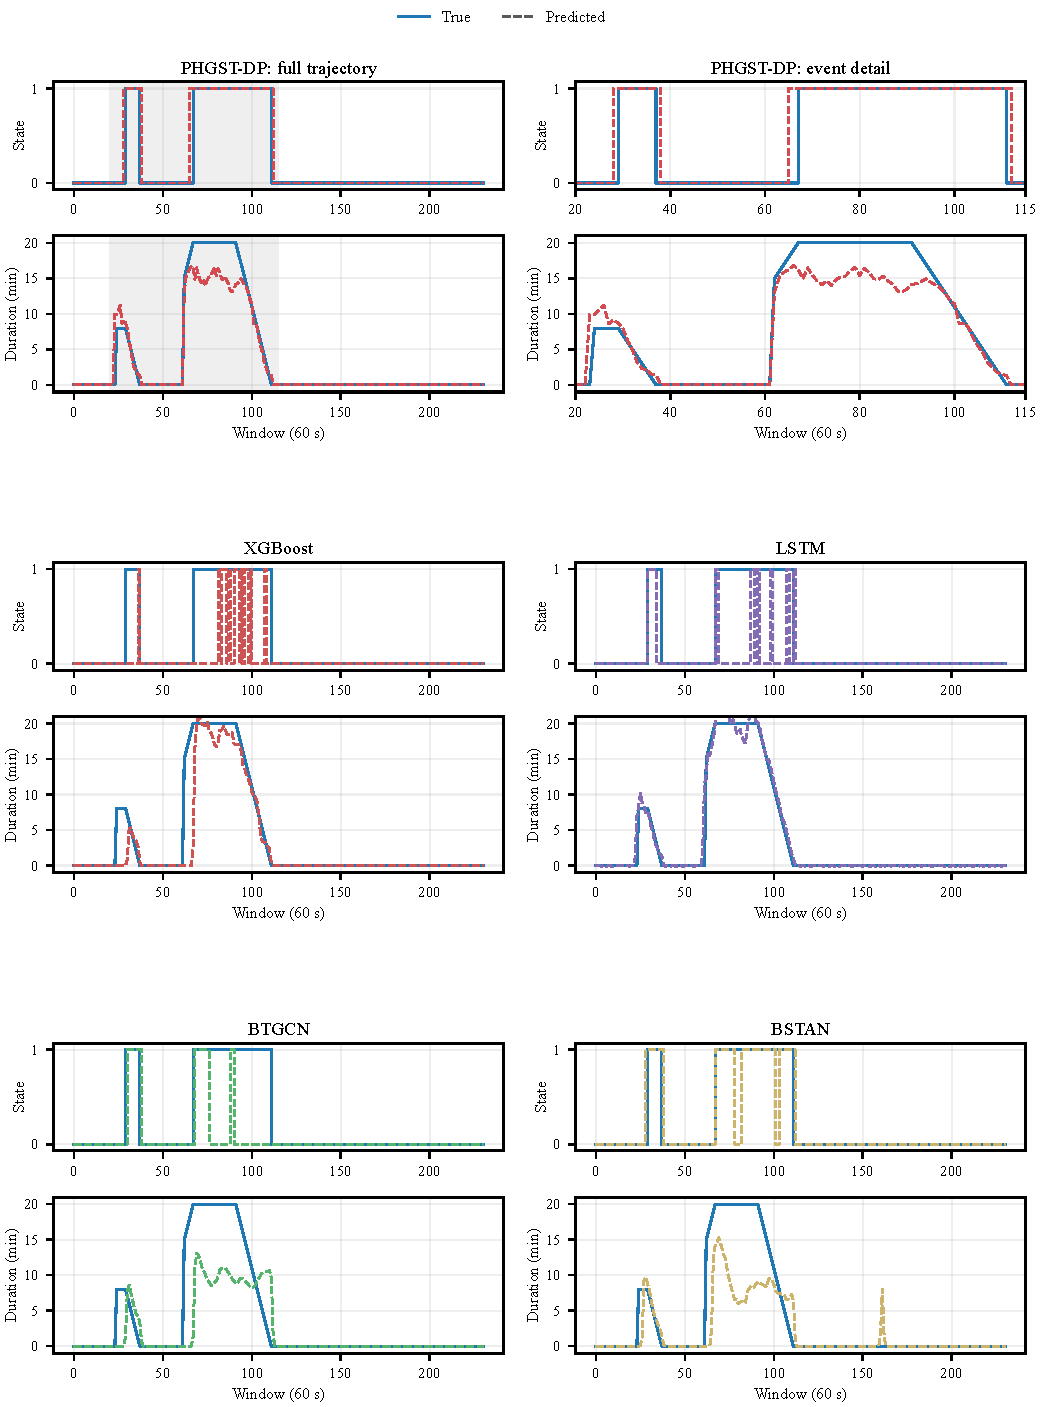
\includegraphics[width=0.96\textwidth,height=0.90\textheight,keepaspectratio]{../figures/key_device_models_aligned.pdf}
\caption{Key-device case for PHGST-DP (upper left), XGBoost, LSTM, BTGCN, and BSTAN on \texttt{num02}, episode \texttt{n10\_human1.0\_\_episode\_03}, Start$\leq5$. Each model has an independent pair: next-window state above and duration over the next 20~min below. Black solid: true; dashed: predicted. The upper-right pair enlarges windows 20--115 (shaded at upper left), using the same vertical scales. Window zero follows the 30-window history.}
\label{fig:key-device-baselines}
\end{figure*}

The all-resource view connects these local traces to coordinated production-state prediction. Figure~\ref{fig:all-devices-main} covers all 15 targets in the same episode, which contains 64 positive bottleneck cells, the highest count among test episodes. PHGST-DP recovers every positive cell of the cutting machine and second welding station (\texttt{num00\_weld\_ws1}), with episode-level State F1 $0.941$. Olive cells denote true positives; coral cells denote false positives and false negatives. The corresponding F1 values are $0.855$ for NoInfo, $0.832$ for NoCluster, and $0.901$ for NoGraph. NoInfo and NoCluster omit the welding-station interval, while NoGraph fragments it. The full model's continuous coverage across both resources illustrates the joint role of resource information, supervision, and graph structure in the production-state report.


\begin{figure*}[t]
\centering
\IfFileExists{../figures/all_devices_state_main.pdf}{%
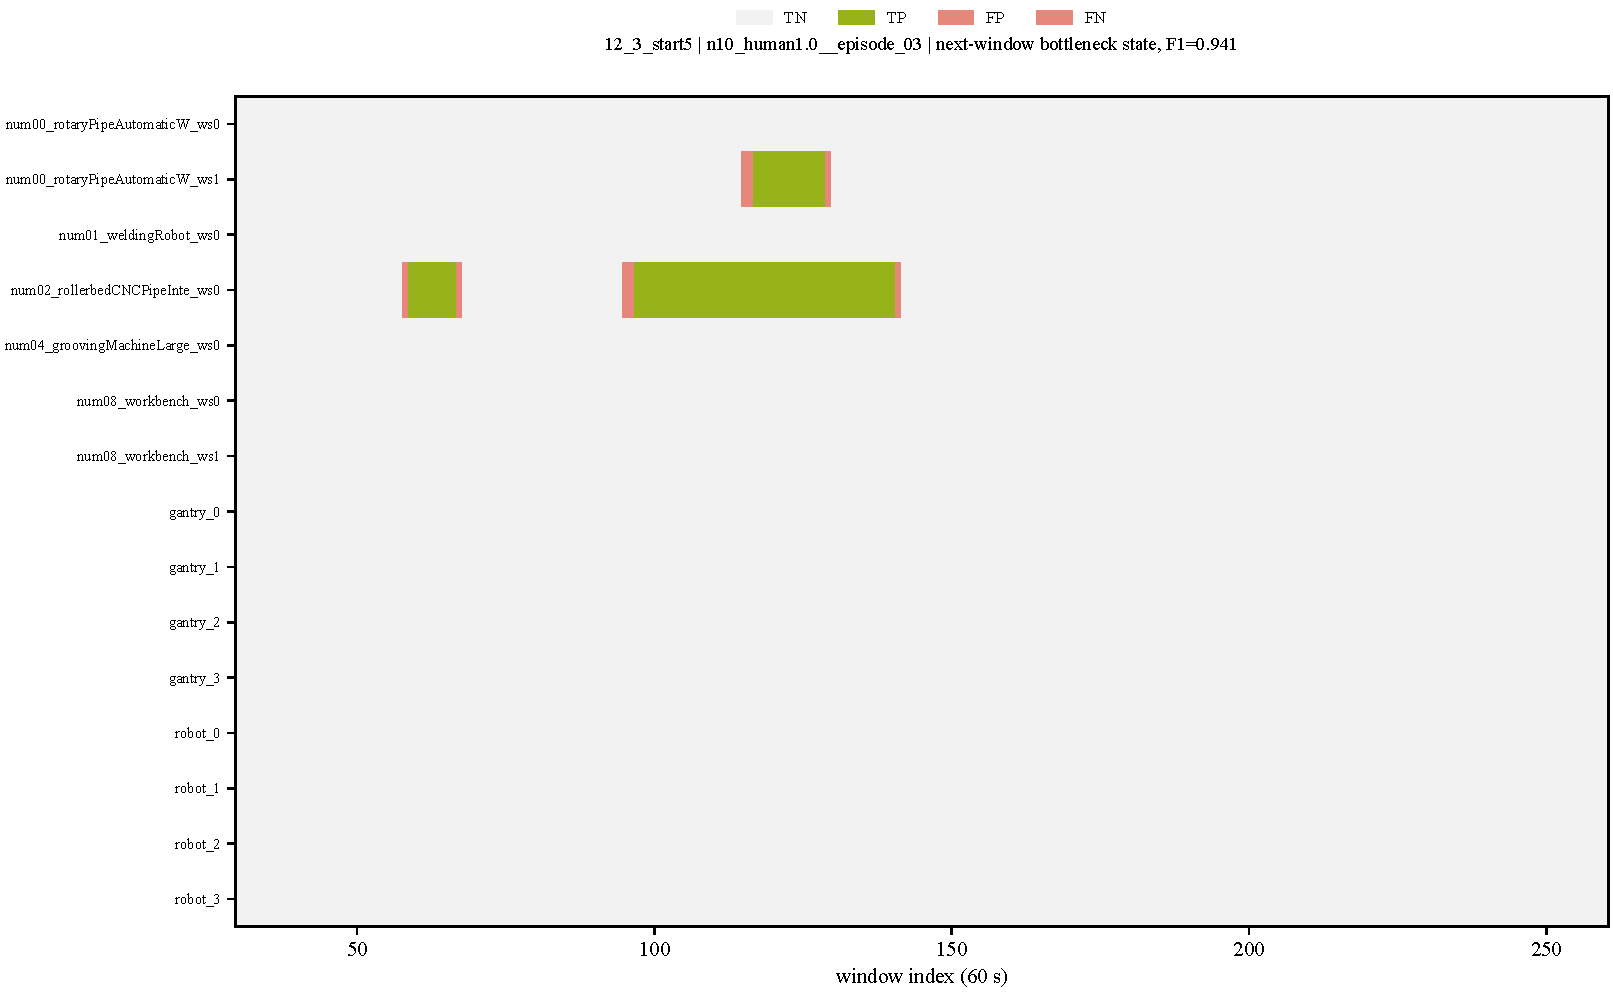
\includegraphics[width=0.96\textwidth]{../figures/all_devices_state_main.pdf}%
}{}
\caption{All-device next-window state map for the retained PHGST-DP on the representative episode (olive: true positive; coral: false positive and false negative). The source render does not separate false positives from false negatives, so both are shown in coral.}
\label{fig:all-devices-main}
\end{figure*}

On the full Start$\leq5$ test split, support is uneven across the 15 targets (Figure~\ref{fig:per-device}). The cutting machine contributes 301 true events, while robot~2 and robot~3 contribute none; those two rows are left unscored rather than entered as zero. F1 on the supported devices ranges from $0.535$ on the welding robot to $0.964$ on bench~ws1. This split is a coverage check for one checkpoint, not a claim that every resource family is equally predictable.

\begin{figure*}[t]
\centering
\IfFileExists{../figures/fig_per_device_start5.pdf}{%
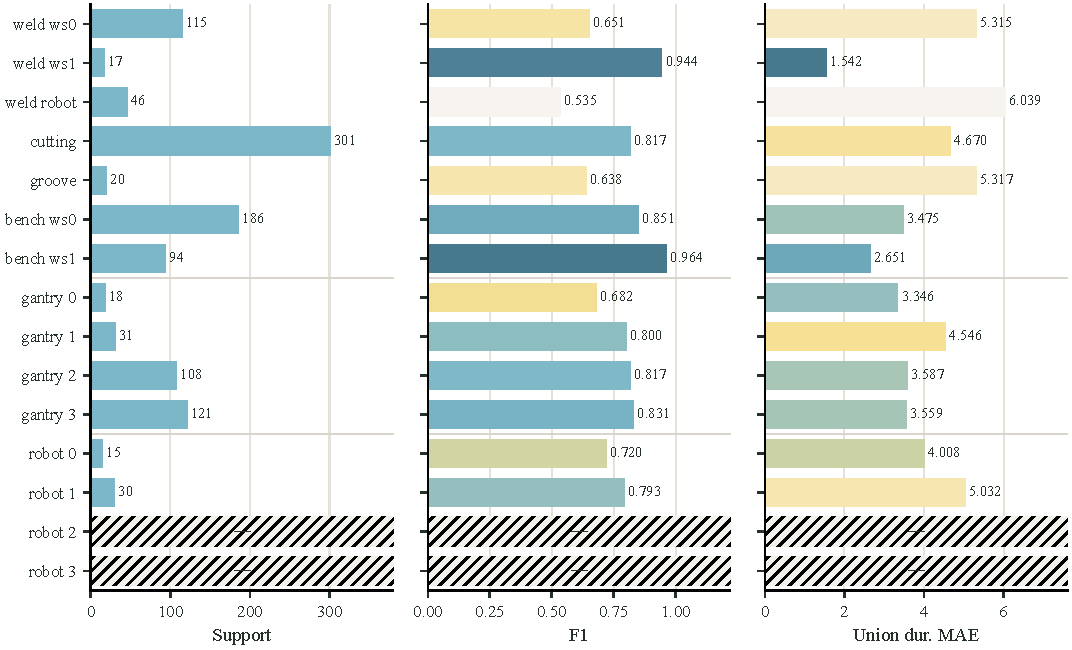
\includegraphics[width=0.96\textwidth]{../figures/fig_per_device_start5.pdf}%
}{}
\caption{Per-device support, F1, and union duration MAE for PHGST-DP at Start$\leq5$ (\texttt{bestmodel\_start5\_seed42}). Colour on F1 and MAE is scaled within that column; support uses one colour because the count is not a quality score. Rows with no true events are hatched and marked with a dash.}
\label{fig:per-device}
\end{figure*}

Process-cause outputs link a predicted event to interpretable production symptoms: transport delay, material shortage, upstream starvation, and queue buildup. The labels encode process-rule evidence, so the explanation is an association with observed operating conditions. Quantitative evaluation covers these four supported classes (Section~\ref{sec:comparison-cause}); blocked-downstream and high-utilization classes have zero test support. Together with the event and state traces, these outputs provide a resource, a time interval, and a process context for reviewing a predicted constraint.


\subsection{Computational efficiency}\label{sec:efficiency}

Computational efficiency was measured for the three retained PHGST-DP checkpoints without retraining, threshold adjustment, or test-set model selection. All measurements used the same NVIDIA GeForce RTX~5090 under Python~3.11.15, PyTorch~2.11.0, and CUDA~12.8. Each checkpoint contains 713,984 trainable parameters and occupies 2.91~MiB. The common test split contains 5,354 windows. A complete test pass used batch size 16 and was repeated five times after 50 warm-up batches. Batch-one forward and report latency were each measured over 5,000 synchronized calls. Forward latency covers the model computation on a GPU-resident batch; report latency additionally includes CPU-to-GPU transfer, prediction, and materialization of the event fields. The test-pass timing further includes DataLoader iteration.


\begin{table*}[t]
\centering
\caption{PHGST-DP inference efficiency on the retained checkpoints. Build time includes test-set construction and is not a weight-loading-only measurement. Test-pass time uses batch size 16; forward and report latency use batch size 1. Latencies are reported as p50/p95/p99.}
\label{tab:efficiency}
\scriptsize
\setlength{\tabcolsep}{3.3pt}
\renewcommand{\arraystretch}{1.08}
\begin{tabular*}{\FullWidth}{@{\extracolsep{\fill}}lrrrrrrr@{}}
\toprule
Start cap & \makecell{Checkpoint\\epoch} & \makecell{Build\\(s)} & \makecell{Test pass\\(s)} & \makecell{Throughput\\(samples/s)} & \makecell{Forward p50/p95/p99\\(ms)} & \makecell{Report p50/p95/p99\\(ms)} & \makecell{Peak GPU\\(MiB)} \\
\midrule
$\leq5$  & 16 & 9.70 & 2.695 & 1,987 & 3.52/4.09/4.24 & 4.75/5.38/5.53 & 175.8 \\
$\leq10$ & 9  & 8.21 & 2.751 & 1,946 & 3.53/4.08/4.21 & 4.77/5.41/5.60 & 175.8 \\
$\leq15$ & 12 & 8.10 & 2.703 & 1,981 & 3.49/4.06/4.16 & 4.72/5.32/5.51 & 175.8 \\
\bottomrule
\end{tabular*}
\end{table*}

Table~\ref{tab:efficiency} shows that the three onset settings have nearly identical inference cost. A complete pass over 5,354 windows takes 2.695--2.751~s, corresponding to 1,946--1,987 samples/s; the throughput spread is only about $2.1\%$. For online batch-one use, the median complete-report latency is 4.72--4.77~ms and the p95 latency is 5.32--5.41~ms. Event decoding and data transfer add approximately 1.2--1.3~ms beyond the pure forward pass. The small variation is expected because changing the onset cap changes the learned checkpoint and decision task but not the PHGST-DP architecture or input shape. The constant 175.8~MiB peak allocated GPU memory and compact checkpoint further indicate that the three forecasting ranges do not introduce additional inference resources.


The largest observed p95 report latency, 5.41~ms, is far below the one-minute sampling interval used by the prediction pipeline. This provides a substantial computation margin for refreshing a bottleneck report after a new window becomes available on the tested platform. The result should nevertheless be interpreted as model-side feasibility rather than end-to-end factory response time: acquisition from MES/WMS and transport systems, feature aggregation, communication, queueing, and downstream decision execution were outside the benchmark. Moreover, the current measurements support within-model comparison across the three PHGST-DP checkpoints only. No matched efficiency measurements are available for the baselines, and the archived runs did not record per-epoch training time, complete fitting time, or process RSS; consequently, no cross-model efficiency ranking or training-cost claim is made.


\section{Discussion}\label{sec:discussion}

PHGST-DP brings bottleneck forecasting closer to the information needed for production intervention: a resource, an expected event interval, an associated process cause, and an order-completion estimate. Its central empirical strength is the combination of advance warning and temporal tracking. Across the three onset caps, Upcoming recall remains above $0.53$, detected-event duration MAE stays below 2~min, and one-step State F1 ranges from $0.883$ to $0.900$. Together, these results describe emerging constraints with enough temporal structure to inform when a resource may need attention and how long its restricted state may persist. The three prediction dimensions serve complementary decisions: event and time outputs identify the constraint, cause outputs provide process context, and remaining-time outputs describe order progress.


The heterogeneous process--logistics representation broadens the evidence available before a target resource becomes constrained. Resource states carry different operational meanings, and grouped embeddings retain those meanings while graph relations connect processing, transport, and supply. In the evaluated ablation configurations, the full model reaches Upcoming recall $0.542$ at Start$\leq5$, compared with $0.104$ for NoGraph and $0.220$ for NoCross (Table~\ref{tab:entity-ablation-new}). The gains concentrate on emerging events, while ongoing-event recognition remains high across configurations. This pattern supports using cross-resource context to recognize precursors and extends the prediction task to gantries and transport robots as well as machines.


Process-informed supervision gives the report an interpretable connection to production conditions. The cause head identifies several supported symptoms with high class recall, while the matched-budget component study shows that cause supervision substantially improves cause accuracy with little change in station identification. Rule-based event construction and regime clustering contribute structured supervision at complementary levels. In the retained label-validity analysis, the exploratory replay places Ops highest on all reported soft service-sensitivity alignment measures. This evidence motivates labels that retain a clear relationship to resource operating conditions, while its pilot scale precludes a general claim that Ops is superior on every notion of label quality. The cause categories express rule-derived process associations; the replay separately evaluates simulated intervention sensitivity.


Delay-pattern conditioning connects these heterogeneous observations across time. Matching recent patches to recurrent patterns supplies temporal context to geographic attention, allowing earlier resource states to inform later bottleneck formation. For events starting more than 10~min ahead, strict report recall is $0.433$ for PHGST-DP and $0.163$ for NoPattern (Table~\ref{tab:delay-ablation-new}). Separate onset and continuation decisions further focus warning on resources that are not yet constrained. These results are consistent with the intended role of the delay module: representing precursors whose consequences emerge after a lag. The aligned case traces provide a direct view of how this predictive information appears as an event trajectory.


The digital-twin evaluation establishes this reporting capability for the studied resource layout, product mix, and 20-min prediction horizon. Deployment can build on the same interface by mapping MES, WMS, and transport-dispatch observations to the resource graph and updating the report as new windows arrive. The measurements in Section~\ref{sec:efficiency} show that model-side report generation fits comfortably within the one-minute update interval on the tested hardware. Further validation can extend to end-to-end data and decision latency, missing or delayed observations, additional seeds and layouts, and the scheduling or throughput outcomes of acting on the forecasts. These directions connect the demonstrated predictive capability to its use in production control.


\section{Conclusion}\label{sec:conclusion}

This study addresses dynamic bottleneck prediction in a production line with interacting processing and logistics resources. PHGST-DP combines a heterogeneous process--logistics graph, process-informed event and cause supervision with regime clustering, and delay-pattern conditioning in a spatiotemporal Transformer. The resulting report integrates bottleneck occurrence and timing, process-cause prediction, and order-completion remaining time. This design connects multi-resource observations to forecasts of where a constraint will develop, when it will emerge, and how it will persist.


Across onset caps of 5, 10, and 15~min, PHGST-DP achieves Report F1 of $0.804/0.778/0.768$, Upcoming recall of $0.542/0.535/0.537$, and detected-event duration MAE of $1.863/1.788/1.716$~min. One-step State F1 reaches $0.883$--$0.900$. Component analyses connect these results to cross-resource information, process-informed supervision, and temporal pattern context, while the case study shows how the outputs track bottleneck onset, persistence, and recovery. PHGST-DP thus provides an integrated and interpretable forecast of production constraints, with temporal detail that supports the planning of timely resource interventions.


%% ========================================================================
%% Bibliography
%% ========================================================================

\bibliographystyle{unsrtnat}
\bibliography{../cas-refs}

\end{document}
